% !TEX root = ../thesis.tex
%
\chapter{External Prior Guided Internal Prior Learning for Real Noisy Image Denoising}
\label{sec:guided}

\section{Learning External Nonlocal Self-Similarity Priors}
\label{sec:system:intro}

Image denoising is a crucial and indispensable step to improve image quality in digital imaging systems. In particular, with the decrease of size of CMOS/CCD sensors, image is more easily to be corrupted by noise and hence denoising is becoming increasingly important for high resolution imaging. The problem of image denoising has been extensively studied in literature and numerous image denoising methods
\cite{bayesshrink,curvelet,ksvd,lssc,ncsr,bm3d,cbm3d,
zhou2012nonparametric,Tomasi1998,blsgsm,nlm,nlbayes,wnnm,pgpd,foe,epll,
mlp,xie2012image,dncnn,
barbu2009training,csf,chen2015learning,Fadili,salmon2014,
Foipractical,Luisier,makitalo2013optimal,Montagner,
jiang2014mixed,Hu2016,xuaccv2016,
fullyblind,rabie2005robust,Liu2008,almapg,noiseclinic,
ncwebsite,Zhu_2016_CVPR,crosschannel2016,neatimage}
have been proposed in the past decades. Most of existing denoising methods focus on the scenario of additive white Gaussian noise (AWGN) 
\cite{bayesshrink,curvelet,ksvd,lssc,ncsr,bm3d,cbm3d,
zhou2012nonparametric,Tomasi1998,blsgsm,nlm,nlbayes,wnnm,pgpd,foe,epll,
mlp,xie2012image,dncnn,barbu2009training,csf,chen2015learning}, where the observed noisy image $\mathbf{y}$ is modeled as the addition of clean image $\mathbf{x}$ and AWGN $\mathbf{n}$, i.e., $\mathbf{y}=\mathbf{x}+\mathbf{n}$. There are also methods proposed for removing Poisson noise \cite{Fadili,salmon2014}, mixed Poisson and Gaussian noise \cite{Foipractical,Luisier,makitalo2013optimal,Montagner}, mixed Gaussian and impulse noise \cite{jiang2014mixed,Hu2016,xuaccv2016}, and realistic noise in real photography \cite{fullyblind,rabie2005robust,Liu2008,almapg,Zhu_2016_CVPR,noiseclinic,
ncwebsite,crosschannel2016,neatimage}.

Natural images have many properties, such as sparsity and nonlocal self-similarity, which can be employed as useful priors for designing image denoising methods. Based on the facts that natural images will be sparsely distributed in some transformed domain, wavelet \cite{bayesshrink} and curvelet \cite{curvelet} transforms have been widely adopted for image denoising. The sparse representation based methods \cite{ksvd,lssc,ncsr,bm3d,cbm3d,
zhou2012nonparametric} encode image patches over a dictionary by using $\ell_{1}$-norm minimization to enforce the sparsity. The well-known bilateral filters \cite{Tomasi1998} employ the prior information that image pixels exhibit similarity in both spatial domain and intensity domain. Other image priors such as multiscale self-similarity \cite{blsgsm} and nonlocal self-similarity \cite{nlm,nlbayes}, or the combination of multiple image priors \cite{wnnm,pgpd} have also been successfully used in image denoising. For example, by using low-rank minimization to characterize the image nonlocal self-similarity, the WNNM \cite{wnnm} method achieves state-of-the-art performance for AWGN denoising. 

Instead of using predefined image priors, methods have also been proposed to learn priors from natural images for denoising. The generative image prior learning methods usually learn prior models from a set of external clean images and apply the learned prior models to the given noisy image \cite{foe,epll,pgpd}, or learn priors from the given noisy image to perform denoising \cite{ksvd}. Recently, the discriminative image prior learning methods \cite{mlp,xie2012image,dncnn,
chen2015learning,
barbu2009training,csf}, which learn denoising models from pairs of clean and noisy images, have been becoming popular. The representative methods include the neural network based methods \cite{mlp,xie2012image,dncnn}, random fields based methods \cite{barbu2009training,csf}, and reaction diffusion based methods \cite{chen2015learning}.
 
\begin{figure}
    \centering
    \begin{subfigure}[t]{0.19\textwidth}
        \centering
        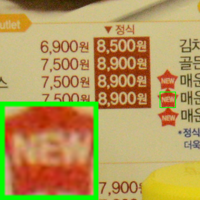
\includegraphics[width=1\textwidth]{images/guided/resize_br_Noisy_CC_Noisy_Nikon_D800_ISO_3200_A3_66.png}
	   \caption{Noisy 33.30}
    \end{subfigure}
    \hfill
    \begin{subfigure}[t]{0.19\textwidth}
        \centering
        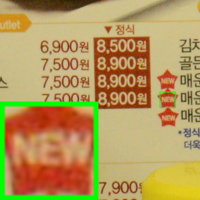
\includegraphics[width=1\textwidth]{images/guided/resize_br_CBM3D_CC_Noisy_Nikon_D800_ISO_3200_A3_66.png}
		\caption{CBM3D34.55}
    \end{subfigure}
    \hfill
    \begin{subfigure}[t]{0.19\textwidth}
        \centering
        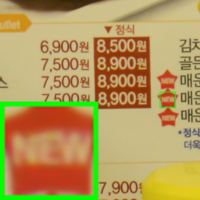
\includegraphics[width=1\textwidth]{images/guided/resize_br_WNNM_CC_Noisy_Nikon_D800_ISO_3200_A3_66.png}
		\caption{WNNM35.85}
    \end{subfigure}
    \hfill
    \begin{subfigure}[t]{0.19\textwidth}
        \centering
        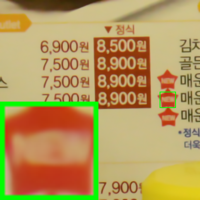
\includegraphics[width=1\textwidth]{images/guided/resize_br_CSF_CC_Noisy_Nikon_D800_ISO_3200_A3_66.png}
		\caption{CSF 35.39}
    \end{subfigure}
    \hfill
    \begin{subfigure}[t]{0.19\textwidth}
        \centering
        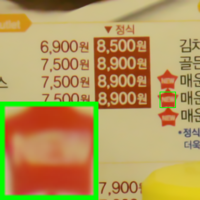
\includegraphics[width=1\textwidth]{images/guided/resize_br_TRD_CC_Noisy_Nikon_D800_ISO_3200_A3_66.png}
		\caption{TNRD 35.97}
    \end{subfigure}
    \hfill
    \begin{subfigure}[t]{0.19\textwidth}
        \centering
        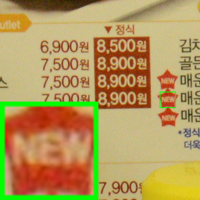
\includegraphics[width=1\textwidth]{images/guided/resize_br_DnCNN_CC_Noisy_Nikon_D800_ISO_3200_A3_66.png}
	   \caption{DnCNN34.14}
    \end{subfigure}
    \hfill
    \begin{subfigure}[t]{0.19\textwidth}
        \centering
        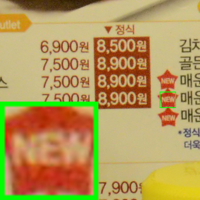
\includegraphics[width=1\textwidth]{images/guided/resize_br_NI_CC_Noisy_Nikon_D800_ISO_3200_A3_66.png}
		\caption{NI 34.39}
    \end{subfigure}
    \hfill
    \begin{subfigure}[t]{0.19\textwidth}
        \centering
        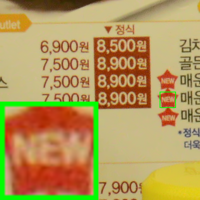
\includegraphics[width=1\textwidth]{images/guided/resize_br_NC_CC_Noisy_Nikon_D800_ISO_3200_A3_66.png}
		\caption{NC 35.33}
    \end{subfigure}
    \hfill
    \begin{subfigure}[t]{0.19\textwidth}
        \centering
        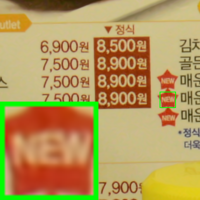
\includegraphics[width=1\textwidth]{images/guided/resize_br_Guided_CC_Noisy_Nikon_D800_ISO_3200_A3_66.png}
		\caption{Ours \textbf{37.49}}
    \end{subfigure}
    \hfill
    \begin{subfigure}[t]{0.19\textwidth}
        \centering
        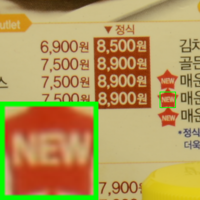
\includegraphics[width=1\textwidth]{images/guided/resize_br_Mean_CC_Noisy_Nikon_D800_ISO_3200_A3_66.png}
		\caption{Mean Image}
    \end{subfigure}
    \caption{Denoised images and PSNR (dB) results of a region cropped from the real noisy image ``Nikon D800 ISO 3200 A3'' \cite{crosschannel2016} by different methods.\ The scene was shot 500 times with the same camera and camera setting.\ The mean image of the 500 shots is roughly taken as the ``ground truth'', with which the PSNR index can be computed. The images are better viewed by zooming in on screen.}
    \label{fig3-1}
\end{figure}

Most of the above mentioned methods focus on AWGN removal, however, the assumption of AWGN is too ideal to be true for real-world noisy images, where the noise is much more complex and varies with different scenes, cameras and camera settings (ISO, shutter speed, and aperture, etc.) \cite{crosschannel2016,healey1994radiometric}. As a result, many denoising methods in literature, including those learning based methods, become less effective when applied to real-world noisy images. Fig. \ref{fig1} shows an example, where we apply some representative and state-of-the-art denoising methods, including CBM3D \cite{cbm3d}, WNNM \cite{wnnm}, DnCNN \cite{dncnn}, CSF \cite{csf}, and TNRD \cite{chen2015learning} to a real noisy image (captured by a Nikon D800 camera with ISO is 3200) provided in \cite{crosschannel2016}. One can see that these methods either remain much the noise or over-smooth the image details.

There have been a few methods \cite{fullyblind,rabie2005robust,Liu2008,almapg,crosschannel2016,Zhu_2016_CVPR,noiseclinic,ncwebsite} and software toolboxes \cite{neatimage} developed for real noisy image denoising. Almost all of these methods follow a two-stage framework: first estimate the parameters of the noise model (usually assumed to be Gaussian or mixture of Gaussians (MoG)), and then perform denoising with the estimated noise model. However, the noise in real noisy images is very complex and is hard to be modeled by explicit distributions such as Gaussian and MoG. According to \cite{healey1994radiometric}, the noise corrupted in the in-camera imaging process \cite{tsin2001statistical,NewInCamera,crosschannel2016,karaimer_brown_ECCV_2016} is signal dependent and comes from five main sources: photon shot, fixed pattern, dark current, readout, and quantization noise. The existing methods \cite{fullyblind,rabie2005robust,Liu2008,almapg,crosschannel2016,Zhu_2016_CVPR,noiseclinic,
ncwebsite,neatimage} mentioned above may not perform well on real noisy image denoising tasks. Fig. \ref{fig3-1} also shows the denoising results of two real noisy image denoising methods, Noise Clinic \cite{noiseclinic,ncwebsite} and Neat Image \cite{neatimage}. One can see that these two methods still generate much noise caused artifacts. 

This work aims to develop a new paradigm for real noisy image denoising. Different from existing real noisy image denoising methods \cite{fullyblind,rabie2005robust,Liu2008,almapg,crosschannel2016,Zhu_2016_CVPR,noiseclinic,ncwebsite}  which focus on noise modeling, we focus on image prior learning. We argue that with a strong and adaptive prior learning scheme, robust denoising performance on real noisy images can still be obtained.  To achieve this goal, we propose to first learn image priors from external clean images, and then employ the learned external priors to guide the learning of internal priors from the given noisy image. The flowchart of the proposed method is illustrated in Fig. \ref{fig3-2}. We first extract millions of patch groups (PGs) from a set of high quality natural images, with which a Gaussian Mixture Model (GMM) is learned as the external image prior. The learned GMM prior model is used to cluster the PGs extracted from the given noisy image, and then an external-internal hybrid orthogonal dictionary is learned as the final prior for each cluster, with which the denoising can be readily performed by weighted sparse coding with closed form solution. Our proposed denoising method is simple and efficient, yet our extensive experiments on real noisy images demonstrate its better denoising performance than the current state-of-the-arts.


\begin{figure}
\label{fig3-2}
\centering
\captionsetup{justification=centering,margin=0.1cm}
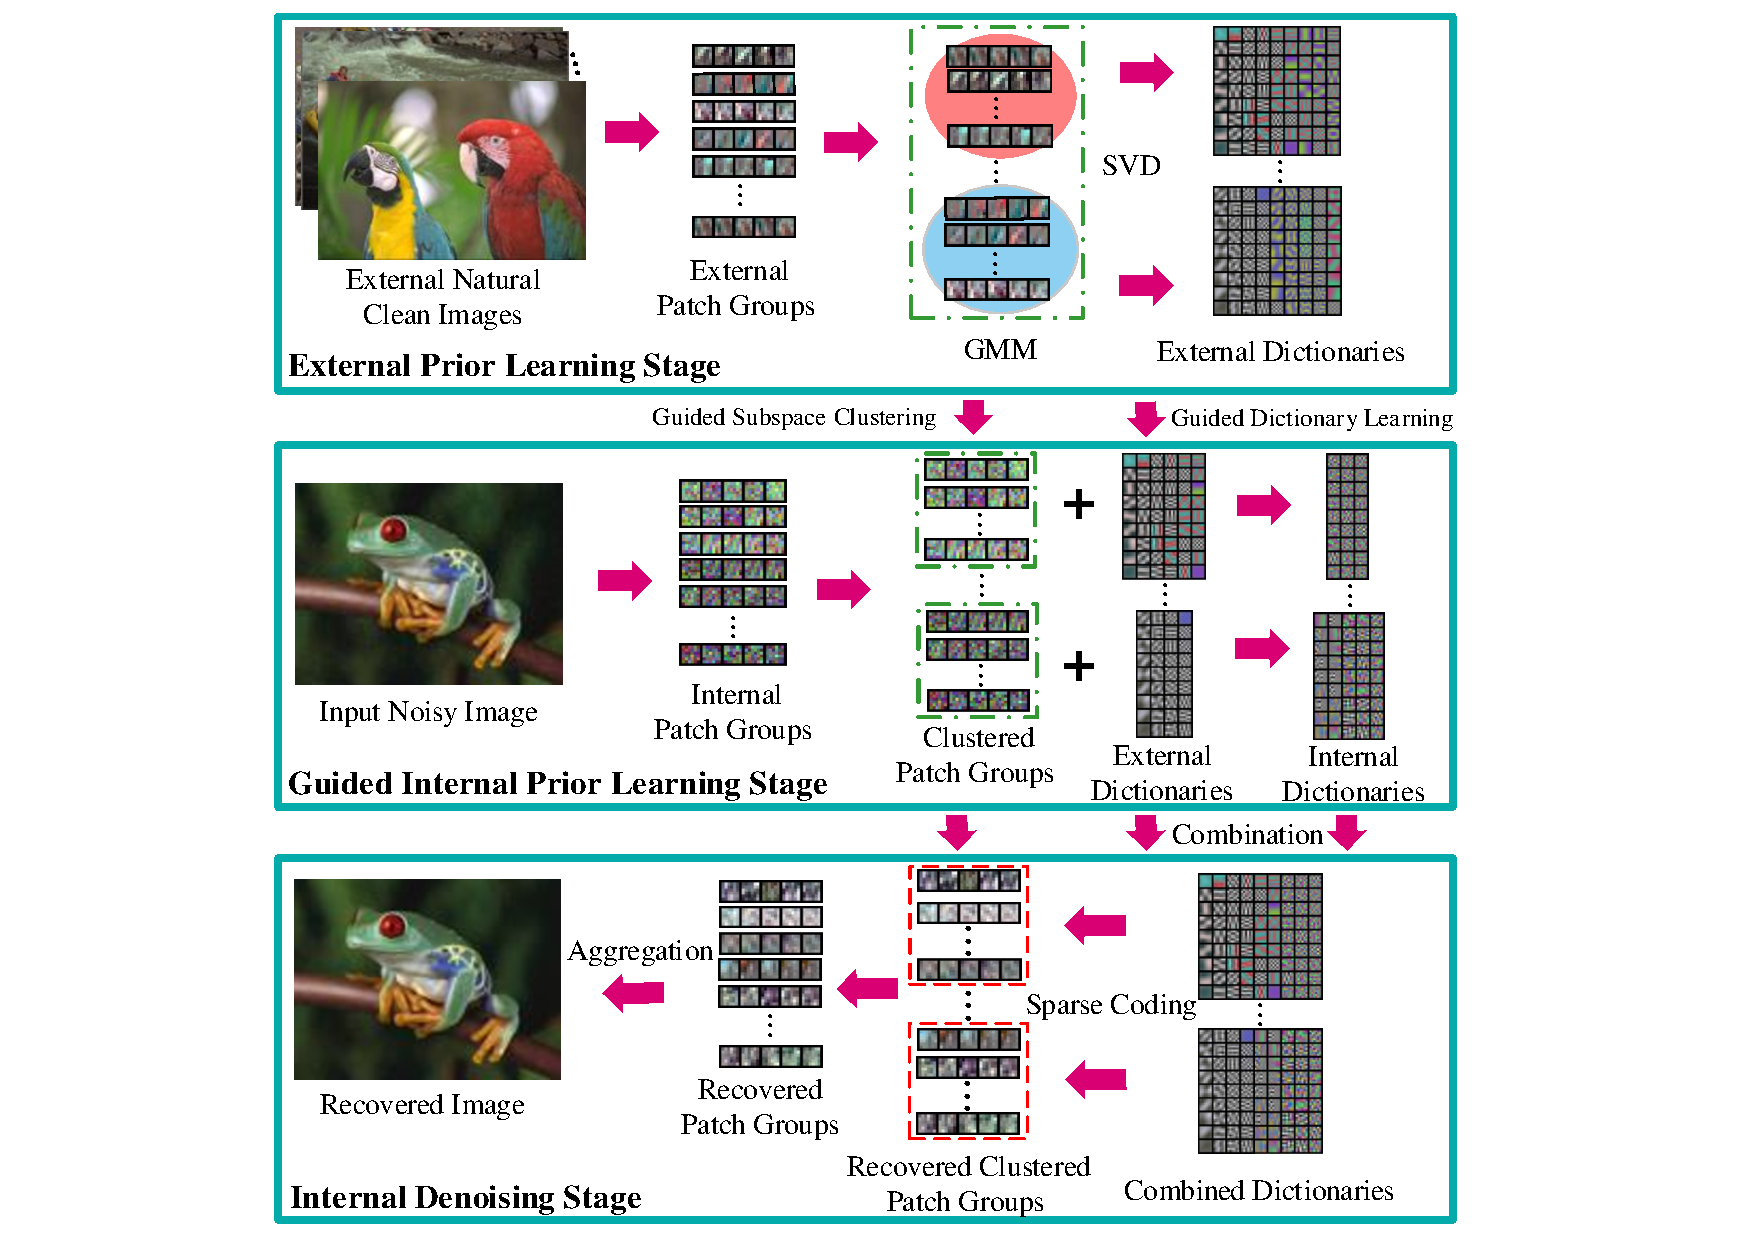
\includegraphics[width=0.8\linewidth]{images/guided/Flowchart.jpg}
\centering
\caption{Flowchart of the proposed external prior guided internal prior learning and denoising framework.}
\end{figure}



\section{Related Work}

\subsection{Internal and External Prior Learning}

Learning natural image priors plays a key role in image denoising
\cite{blsgsm,
zhou2012nonparametric,ksvd,lssc,ncsr,foe,epll,pgpd,mlp,xie2012image,dncnn,
barbu2009training,csf,chen2015learning}. There are mainly three categories of prior learning based methods. 1) External prior learning methods \cite{foe,epll,pgpd} learn priors (e.g., dictionaries) from a set of external clean images, and the learned priors are used to recover the latent clean image from the given noisy image. 2) Internal prior learning methods \cite{blsgsm,zhou2012nonparametric,ksvd,lssc,ncsr} directly learn priors from a given noisy image, and image denoising is often done simultaneously with the prior learning process. 3) Discriminative prior learning methods \cite{mlp,xie2012image,dncnn,barbu2009training,
csf,chen2015learning} learn discriminative models or mapping functions from clean and noisy image pairs, and the learned models or mapping functions are applied to a noisy image for denoising. This paper focuses on the first two categories of prior learning methods, which belongs to generative prior learning methods. 

It has been shown \cite{foe,epll,pgpd} that the external priors learned from natural clean images are effective and efficient for universal image denoising problems, whereas they are not adaptive to the given noisy image and some fine-scale image structures may not be well recovered. By contrast, the internal priors learned from the given noisy image are adaptive to image content, but the learned priors can be much affected by noise and the learning processing is usually slow. In addition, most of the internal prior learning methods \cite{blsgsm,zhou2012nonparametric,ksvd,lssc,ncsr} assume AWGN noise, making the learned priors less robust for real noisy images. In this paper, we use external priors to guide the internal prior learning. Our method is not only much faster than the traditional internal learning methods, but also very robust to denoise real noisy images.


\subsection{Real Noisy Image Denoising}

Most of the denoising methods in literature \cite{bayesshrink,curvelet,ksvd,lssc,ncsr,bm3d,cbm3d,
zhou2012nonparametric,Tomasi1998,blsgsm,nlm,nlbayes,wnnm,pgpd,foe,epll,
mlp,xie2012image,dncnn,barbu2009training,csf,chen2015learning} assume AWGN noise and use simulated noisy images for algorithm design and evaluation. Recently, several denoising methods have been proposed to remove unknown noise from real-world noisy images \cite{fullyblind,rabie2005robust,Liu2008,almapg,crosschannel2016,Zhu_2016_CVPR,noiseclinic,ncwebsite}. Portilla \cite{fullyblind} employed a correlated Gaussian model to estimate the noise of each wavelet subband. Rabie \cite{rabie2005robust} modeled the noisy pixels as outliers and performed denoising via Lorentzian robust estimator. Liu et al. \cite{Liu2008} proposed the ``noise level function'' to estimate the noise and performed denoising by learning a Gaussian conditional random field. Gong et al. \cite{almapg} proposed to model the data fitting term via weighted sum of $\ell_{1}$ and $\ell_{2}$ norms and performed denoising by a simple sparsity regularization term in the wavelet transform domain. The ``Noise Clinic'' \cite{noiseclinic,ncwebsite} estimates the noise distribution by using a multivariate Gaussian model and removes the noise by using a generalized version of nonlocal Bayesian model \cite{nlbayes}. Zhu et al. \cite{Zhu_2016_CVPR} proposed a Bayesian method to approximate and remove the noise via a low-rank mixture of Gaussians (MoG) model. The method in \cite{crosschannel2016} models the cross-channel noise in real noisy image as a multivariate Gaussian and the noise is removed by the Bayesian nonlocal means filter \cite{kervrann2007bayesian}. The commercial software Neat Image \cite{neatimage} estimates the noise parameters from a flat region of the given noisy image and filters the noise correspondingly. 


The methods \cite{fullyblind,rabie2005robust,Liu2008,almapg,crosschannel2016,Zhu_2016_CVPR,noiseclinic,ncwebsite} mentioned above emphasize much on the noise modeling, and they use Gaussian or MoG to model the noise in real noisy images. Nonetheless, the noise in real noisy images is very complex and hard to be modeled by explicit distributions \cite{healey1994radiometric}. These works ignore the importance of learning image priors, which actually can be easier to model compared with modeling the complex realistic noise. In this paper, we propose a simple yet effective image prior learning method for real noisy image denoising. Due to its strong prior modeling ability, the proposed method simply models the noise as locally Gaussian, and it achieves highly competitive performance on real noisy image denoising.


\section{External Prior Guided Internal Prior Learning for Image Denoising}

In this section, we first describe the learning of external prior, and then describe in detail the guided internal prior learning method, followed by the denoising algorithm.

\subsection{Learn External Patch Group Priors}

The nonlocal self-similarity based patch group (PG) prior learning \cite{pgpd} has proved to be very effective for image denosing. In this work, we extract PGs from natural clean images to learn external priors. A PG is a group of similar patches to a local patch. In our method, each local patch is extracted from a RGB image with patch size $p\times p \times 3$.\ We search the $M$ most similar (i.e., smallest Euclidean distance) patches to this local patch (including the local patch itself) in a $W\times W$ region around it. Each patch is stretched to a patch vector $\mathbf{x}_{m}\in \mathbb{R}^{3p^{2}\times1}$ to form the PG, denoted by $\{\mathbf{x}_{m}\}_{m=1}^{M}$.\ The mean vector of this PG is $\bm{\mu}=\frac{1}{M}\sum_{m=1}^{M}\mathbf{x}_{m}$, and the group mean subtracted PG is defined as $\mathbf{\overline{X}}\triangleq \{\mathbf{\overline{x}}_{m}=\mathbf{x}_{m}-\bm{\mu}\}_{m=1}^{M}$.

Assume that a number of $L$ PGs are extracted from a set of external natural images, and the $l$-th PG is $\mathbf{\overline{X}}_{l}\triangleq \{\mathbf{\overline{x}}_{l,m}\}_{m=1}^{M}, l=1,...,L$.\ A Gaussian Mixture Model (GMM) is learned to model the PG prior.\ The overall log-likelihood function is
\vspace{-2mm}
\begin{equation}\label{equ3-1}
\vspace{-2mm}
\begin{split}
\ln\mathcal{L}=\sum_{l=1}^{L} \ln(\sum_{k=1}^{K}\pi_{k}\prod_{m=1}^{M}\mathcal{N}(\mathbf{\overline{x}}_{l,m}|\bm{\mu}_{k},\bm{\Sigma}_{k})).
\end{split}
\end{equation}
The learning process is similar to the GMM learning in \cite{pgpd,epll}.\ Finally, a GMM model with $K$ Gaussian components is learned, and the learned parameters include mixture weights $\{\pi_{k}\}_{k=1}^{K}$, mean vectors $\{\bm{\mu}_{k}\}_{k=1}^{K}$, and covariance matrices $\{\bm{\Sigma}_{k}\}_{k=1}^{K}$.\ Note that the mean vector of each cluster is naturally zero, i.e., $\bm{\mu}_{k}=\bm{0}$.  

To better describe the subspace of each Gaussian component, we perform singular value decomposition (SVD) \cite{eckart1936approximation} on the covariance matrix:
\vspace{-2mm}
\begin{equation}\label{equ3-2}
\vspace{-2mm}
\bm{\Sigma}_{k}=\bm{U}_{k}\bm{S}_{k}\bm{U}_{k}^{\top}.
\end{equation}
The eigenvector matrices $\{\bm{U}_{k}\}_{k=1}^{K}$ will be employed as the external orthogonal dictionary to guide the internal sub-dictionary learning in next sub-section.\ The singular values in $\bm{S}_{k}$ reflect the significance of the singular vectors in $\bm{U}_{k}$.\ They  will also be utilized as prior weights for weighted sparse coding in our denoising algorithm.


\subsection{Guided Internal Prior Learning}

After the external PG prior model is learned from external natural clean images, we employ it to guide the internal PG prior learning for a given real noisy image.\ The guidance lies in two aspects. First, the external prior will guide the subspace clustering of internal noisy PGs. Second, the external prior will guide the orthogonal dictionary learning of internal noisy PGs.

\subsubsection{Internal Subspace Clustering}

Given a real noisy image $\mathbf{y}$, we extract $N$ (overlapped) local patches from it.\ Similar to the external prior learning stage, for the $n$-th ($n=1,...,N$) local patch we search its $M$ most similar (by Euclidean distance) patches around it to form a noisy PG, denoted by $\bm{Y}_{n} = \{\mathbf{y}_{n,1},...,\mathbf{y}_{n,M}\}$.\ Then the group mean of $\bm{Y}_{n}$, denoted by $\bm{\mu}_{n}$, is subtracted from each patch by $\bm{\overline{y}}_{n,m}\triangleq\mathbf{y}_{n,m}-\bm{\mu}_{n}$, leading to the mean subtracted noisy PG $\bm{\overline{Y}}_{n}\triangleq \{\bm{\overline{y}}_{n,m}\}_{m=1}^{M}$.

The external GMM prior models $\{\mathcal{N}(\bm{0},\bm{\Sigma}_{k})\}_{k=1}^{K}$ basically characterize the subspaces of natural high quality PGs.\ Therefore, we project each noisy PG $\bm{\overline{Y}}_{n}$ into the subspaces of $\{\mathcal{N}(\bm{0},\bm{\Sigma}_{k})\}_{k=1}^{K}$ and assign it to the most suitable subspace based on the posterior probability:
\vspace{-2mm}
\begin{equation}\label{equ3-3}
\vspace{-2mm}
P(k|\bm{\overline{Y}}_{n})=\frac{\prod_{m=1}^{M}\mathcal{N}(\bm{\overline{y}}_{n,m}|\bm{0},\bm{\Sigma}_{k})}{\sum_{l=1}^{K}\prod_{m=1}^{M}\mathcal{N}(\bm{\overline{y}}_{n,m}|\bm{0},\bm{\Sigma}_{l})}
\end{equation}
for $k=1,...,K$.\ Then $\bm{\overline{Y}}_{n}$ is assigned to the subspace with the maximum \emph{a}-posteriori (MAP) probability $\max_{k}P(k|\bm{\overline{Y}}_{n})$.


\subsubsection{Guided Orthogonal Dictionary Learning}

Assume that we have assigned all the internal noisy PGs $\{\bm{\overline{Y}}_{n}\}_{n=1}^{N}$ to their corresponding most suitable subspaces in $\{\mathcal{N}(\bm{0},\bm{\Sigma}_{k})\}_{k=1}^{K}$. For the $k$-th subspace, the noisy PGs assigned to it are $\{\bm{\overline{Y}}_{k_{n}}\}_{n=1}^{N_{k}}$, where $\bm{\overline{Y}}_{k_{n}}=[\bm{\overline{y}}_{k_{n},1},...,\bm{\overline{y}}_{k_{n},M}]$ and $\sum_{k=1}^{K}N_{k}=N$.\ We propose to learn an orthogonal dictionary $\bm{D}_{k}$ from each set of PGs $\bm{\overline{Y}}_{k_{n}}$ to characterize the internal PG prior with the guidance of the corresponding external orthogonal dictionary $\bm{U}_{k}$ (Eq.\ (\ref{equ2})). The reasons that we learn orthogonal dictionaries are two-fold.\ Firstly, the PGs $\{\bm{\overline{Y}}_{k_{n}}\}_{n=1}^{N_{k}}$ are in a subspace of the whole space of all PGs; therefore, there is no necessary to learn a redundant over-complete dictionary to characterize it, while an orthonormal dictionary has naturally zero \emph{mutual incoherence} \cite{donoho2001uncertainty}. Secondly, the orthogonality of dictionary can make the patch encoding in the testing stage very efficient, leading to an efficient denoising algorithm (please refer to sub-section III-C for more details).

We let the orthogonal dictionary $\bm{D}_{k}$ be 
\vspace{-2mm}
\begin{equation}
\vspace{-2mm}
\label{equ3-4}
\bm{D}_{k}\triangleq[\bm{D}_{k,\text{E}}\ \bm{D}_{k,\text{I}}]\in \mathbb{R}^{3p^2\times 3p^2},
\end{equation}
where $\bm{D}_{k,\text{E}}=\bm{U}_{k}(:,1:r)\in\mathbb{R}^{3p^2\times r}$ is the external sub-dictionary and it includes the first $r$ most important eigenvectors of $\bm{U}_{k}$, and the internal sub-dictionary $\bm{D}_{k,\text{I}}\in\mathbb{R}^{3p^2\times (3p^2-r)}$ is to be adaptively learned from the noisy PGs $\{\bm{\overline{Y}}_{k_{n}}\}_{n=1}^{N_{k}}$.\ The rationale to design $\bm{D}_{k}$ as a hybrid dictionary is as follows.\ The external sub-dictionary $\bm{D}_{k,\text{E}}$ is pre-trained from external clean data, and it represents the $k$-th latent subspace of natural images, which is helpful to reconstruct the common latent structures of images. However, $\bm{D}_{k,\text{E}}$ is general to all images but not adaptive to the given noisy image.\ Some fine-scale details specific to the given image may not be well characterized by $\bm{D}_{k,\text{E}}$. Therefore, we learn an internal sub-dictionary $\bm{D}_{k,\text{I}}$ to supplement $\bm{D}_{k,\text{E}}$.\ In other words, $\bm{D}_{k,\text{I}}$ is to reveal the latent subspace adaptive to the input noisy image, which cannot be effectively represented by $\bm{D}_{k,\text{E}}$. 

For notation simplicity, in the following development we ignore the subspace index $k$ for $\bm{\overline{Y}}_{k_{n}}$ and $\bm{D}_{k}$, etc.\ The learning of hybrid orthogonal dictionary $\bm{D}$ is performed under the following weighted sparse coding
framework:
\vspace{-2mm}
\begin{equation}\label{equ3-5}
\vspace{-2mm}
\begin{split}
\min_{\bm{D}_{\text{I}},\{\bm{\alpha}_{n,m}\}}
&\sum_{n=1}^{N}\sum_{m=1}^{M}(\|\bm{\overline{y}}_{n,m}-\bm{D}\bm{\alpha}_{n,m}\|_{2}^{2}+\sum_{j=1}^{3p^{2}}\lambda_{j}|\bm{\alpha}_{n,m,j}|)
\\
&
\text{s.t.}
\quad
\bm{D}=[\bm{D}_{\text{E}}\ \bm{D}_{\text{I}}],\ \bm{D}^{\top}\bm{D} = \bm{I},
\end{split}
\end{equation}
where $\bm{I}$ is the $3p^{2}$ dimensional identity matrix, $\bm{\alpha}_{n,m}$ is the sparse coding vector of the $m$-th patch $\bm{\overline{y}}_{n,m}$ in the $n$-th PG $\bm{\overline{Y}}_{n}$ and $\bm{\alpha}_{n,m,j}$ is the $j$-th element of $\bm{\alpha}_{n,m}$. $\lambda_{j}$ is the $j$-th regularization parameter defined as
\vspace{-2mm}
\begin{equation}\label{equ3-6}
\vspace{-2mm}
\lambda_{j} = \lambda/(\sqrt{\bm{S}_{k}(j)}+\varepsilon),
\end{equation}
where $\bm{S}_{k}(j)$ is the $j$-th singular value of diagonal singular value matrix $\bm{S}_{k}$ (please refer to Eq.\ (\ref{equ3-2})) and $\varepsilon$ is a small positive number to avoid zero denominator.\ Note that $\bm{D}_{\text{E}}=\bm{U}_{k}$ if $r=3p^{2}$ and $\bm{D}_{\text{E}}=\emptyset$ if $r=0$.

In the dictionary learning model (\ref{equ3-5}), we use the $\ell_{2}$ norm to model the representation residual of PGs. This is because the patches in those PGs have similar content, and we assume that the noise therein will have similar statistics, which can be roughly modeled as locally Gaussian. On the other hand, this will make the dictionary learning much easier to solve. We employ an alternating iterative approach to solve the optimization problem (\ref{equ3-5}). Specifically, we initialize the orthogonal dictionary as $\bm{D}^{(0)}=\bm{U}_{k}$ and for $t=0,1, ...,T-1$, and alternatively update $\bm{\alpha}_{n,m}$ and $\bm{D}_{\text{I}}$ as follows.

\vspace{2mm}
\textbf{Updating Sparse Coding Coefficients}: Given the orthogonal dictionary $\bm{D}^{(t)}$, we update each sparse coding vector $\bm{\alpha}_{n,m}$ by solving
\vspace{-2mm}
\begin{equation}\label{equ3-7}
\vspace{-2mm}
\begin{split}
\bm{\alpha}_{n,m}^{(t+1)}:=\argmin_{\bm{\alpha}_{n,m}}
\|\bm{\overline{y}}_{n,m}-\bm{D}^{(t)}\bm{\alpha}_{n,m}\|_{2}^{2}+\sum_{j=1}^{3p^{2}}\lambda_{j}|\bm{\alpha}_{n,m,j}|.
\end{split}
\end{equation}
Since dictionary $\bm{D}^{(t)}$ is orthogonal, the problems (\ref{equ3-7}) has a closed-form solution
\vspace{-2mm}
\begin{equation}\label{equ3-8}
\bm{\alpha}_{n,m}^{(t+1)}= \text{sgn}((\bm{D}^{(t)})^{\top}\bm{\overline{y}}_{n,m})\odot \text{max}(|(\bm{D}^{(t)})^{\top}\bm{\overline{y}}_{n,m}|-\bm{\lambda},\bm{0}),
\end{equation}
where $\bm{\lambda} = \frac{1}{2}[\lambda_{1},\lambda_{2},...,\lambda_{3p^2}]^{\top}$ is the vector of regularization parameter, $\text{sgn}(\bullet)$ is the sign function and $\odot$ means element-wise multiplication.\ The detailed derivation of Eq. (\ref{equ3-8}) can be found in Appendix A.
 
\vspace{2mm}
\textbf{Updating Internal Sub-dictionary}: Given the sparse coding vectors $\{\bm{\alpha}_{n,m}^{(t+1)}\}$, we update the internal sub-dictionary by solving
\vspace{-2mm}
\begin{equation}\label{equ3-9}
\begin{split}
\bm{D}_{\text{I}}^{(t+1)}
:
&
=
\argmin_{\textbf{D}_{\text{I}}}
\sum_{n=1}^{N}\sum_{m=1}^{M}\|\bm{\overline{y}}_{n,m}-\bm{D}\bm{\alpha}_{n,m}^{(t+1)}\|_{2}^{2}
\\
&
=
\argmin_{\textbf{D}_{\text{I}}}
\|\bm{\overline{Y}}_{n}-\bm{D}\bm{A}^{(t+1)}\|_{F}^{2}
\\
\text{s.t.}
\quad
\bm{D}
&
=
[\bm{D}_{\text{E}}\ \bm{D}_{\text{I}}],\ \bm{D}_{\text{I}}^{\top}\bm{D}_{\text{I}} = \bm{I}_{(3p^2-r)},\ \bm{D}_{\text{E}}^{\top}\bm{D}_{\text{I}} = \bm{0},
\end{split}
\end{equation}
where $\textbf{A}^{(t+1)}=[\bm{\alpha}_{1,1}^{(t+1)},...,\bm{\alpha}_{1,M}^{(t)},...,\bm{\alpha}_{N,1}^{(t+1)},...,\bm{\alpha}_{N,M}^{(t+1)}]$ and $\bm{I}_{(3p^2-r)}$ is the $(3p^2-r)$ dimensional identity matrix.\ The sparse coefficients matrix can be written as $\bm{A}^{(t+1)}=[(\bm{A}_{\text{E}}^{(t+1)})^{\top}\ (\bm{A}_{\text{I}}^{(t+1)})^{\top}]^{\top}$ where the external part $\bm{A}_{\text{E}}^{(t+1)}\in\mathbb{R}^{r\times NM}$ and the internal part $\bm{A}_{\text{I}}^{(t+1)}\in\mathbb{R}^{(3p^2-r)\times NM}$ represent the coding coefficients of $\bm{Y}$ over external sub-dictionary $\bm{D}_{\text{E}}$ and internal sub-dictionary $\bm{D}_{\text{I}}^{(t)}$, respectively.\ According to the following Theorem \ref{th1}, by setting $\mathcal{Y}=\bm{\overline{Y}}_{n}-\bm{D}_{\text{E}}\bm{A}_{\text{E}}^{(t+1)},\mathcal{E}=\bm{D}_{\text{E}},\mathcal{D}=\bm{D}_{\text{I}},\mathcal{A}=\bm{A}_{\text{I}}$, the problem (\ref{equ3-9}) has a closed-form solution $\bm{D}_{\text{I}}^{(t+1)}=\bm{U}_{\text{I}}\bm{V}_{\text{I}}^{\top}$, where $\bm{U}_{\text{I}}\in\mathbb{R}^{3p^2\times (3p^2-r)}$ and $\bm{V}_{\text{I}}\in\mathbb{R}^{(3p^2-r)\times (3p^2-r)}$ are the orthogonal matrices obtained by the following SVD \cite{eckart1936approximation}
\vspace{-1mm}
\begin{equation}\label{equ3-10}
\vspace{-1mm}
(\bm{I}-\bm{D}_{\text{E}}\bm{D}_{\text{E}}^{\top})\bm{Y}(\bm{A}_{\text{I}}^{(t+1)})^{\top}
=
\bm{U}_{\text{I}}\bm{S}_{\text{I}}\bm{V}_{\text{I}}^{\top}.
\end{equation}
The orthogonality of internal sub-dictionary $\bm{D}_{\text{I}}^{(t+1)}$ can be shown by checking that
$(\bm{D}_{\text{I}}^{(t+1)})^{\top}(\bm{D}_{\text{I}}^{(t+1)})=\bm{V}_{\text{I}}\bm{U}_{\text{I}}^{\top}\bm{U}_{\text{I}}\bm{V}_{\text{I}}^{\top}=\bm{I}_{(3p^2-r)}$.\ In fact, the Theorem \ref{th3-1} provides a sufficient and necessary condition to guarantee the existence of the closed-form solution for the internal sub-dictionary of the problem (\ref{equ3-9}).

\begin{theorem}
\label{th3-1}
Let $\mathcal{A}\in \mathbb{R}^{(3p^2-r)\times M}$, $\mathcal{Y}\in \mathbb{R}^{3p^2\times M}$ be two given data matrices. $\mathcal{E}\in\mathbb{R}^{3p^2\times r}$ is a given matrix satisfying $\mathcal{E}^{\top}\mathcal{E}=\bm{I}_{r\times r}$, then $\hat{\mathcal{D}} = \mathcal{U}\mathcal{V}^{\top}$ is the necessary condition of
\begin{equation}\label{equ3-11}
\begin{split}
\hat{\mathcal{D}}
=
&
\arg\min_{\mathcal{D}}\|\mathcal{Y}-\mathcal{D}\mathcal{A}\|_{F}^{2}
\quad
\\
&
\text{s.t.}
\quad
\mathcal{D}^{\top}\mathcal{D} = \bm{I}_{(3p^2-r)\times (3p^2-r)}, \mathcal{E}^{\top}\mathcal{D} = \bm{0}_{r\times (3p^2-r)}
,
\end{split}
\end{equation}
where $\mathcal{U}\in \mathbb{R}^{3p^2\times (3p^2-r)}$ and $\mathcal{V}\in \mathbb{R}^{(3p^2-r)\times (3p^2-r)}$ are the orthogonal matrices obtained by performing economy (a.k.a. reduced) SVD  \cite{eckart1936approximation}:
\begin{equation}\label{equ3-12}
(\bm{I}_{3p^2\times 3p^2}-\mathcal{E}\mathcal{E}^{\top})\mathcal{Y}\mathcal{A}^{\top} = \mathcal{U}\Sigma\mathcal{V}^{\top}
\end{equation}
Besides, if $\text{rank}(\Sigma)=3p^2-r$, $\hat{\mathcal{D}} = \mathcal{U}\mathcal{V}^{\top}$ is also the sufficient condition of problem (\ref{equ3-11}). 
\end{theorem}


The proof of the Theorem \ref{th3-1} can be found in Appendix B. Though the problem (\ref{equ3-9}) has a closed-form solution by SVD \cite{eckart1936approximation}, the uniqueness of solution cannot be guaranteed since the matrices $(\bm{I}_{3p^2\times 3p^2}-\mathcal{E}\mathcal{E}^{\top})\mathcal{Y}\mathcal{A}^{\top}$ as well as $\mathcal{U}$ and $\mathcal{V}$ may be reduced to matrices of lower rank. Hence, we also analyze the uniqueness of the solution $\hat{\mathcal{D}}$ by the following Theorem \ref{th3-2}, whose proof can be found in Appendix C.

\begin{theorem}
\label{th3-2}
(a) If $(\bm{I}_{3p^2\times 3p^2}-\mathcal{E}\mathcal{E}^{\top})\mathcal{Y}\mathcal{A}^{\top}\in\mathbb{R}^{3p^2\times (3p^2-r)}$ is nonsingular, i.e., $\text{rank}(\Sigma)=3p^2-r$, then the solution of $\hat{\mathcal{D}}=\mathcal{U}\mathcal{V}^{\top}$ is unique; (b) If $(\bm{I}_{3p^2\times 3p^2}-\mathcal{E}\mathcal{E}^{\top})\mathcal{Y}\mathcal{A}^{\top}$ is singular, i.e., $0\le\text{rank}(\bm{\Sigma})< 3p^2-r$, then the number of possible solutions of $\hat{\mathcal{D}}$ is $2^{3p^2-r-\text{rank}(\bm{\Sigma})}$ for fixed $\mathcal{U}$ and $\mathcal{V}$.
\end{theorem}

The above alternative updating steps are repeated until the number of iterations exceeds a preset threshold. In each step, the energy value of the objective function (\ref{equ3-5}) is decreased and we empirically found that the proposed model usually converges in 10 iterations. We summarize the procedures in Algorithm 1.


\begin{table}\label{alg3-1}\vspace{3mm}
\begin{tabular}{l}
\hline
\textbf{Algorithm 1}: External Prior Guided Internal Prior Learning
\\
\hline
\textbf{Input:} Matrices $\bm{\overline{Y}}_{n}$, external sub-dictionary $\bm{D}_{\text{E}}$, parameter vector $\bm{\lambda}$
\\
\textbf{Initialization:} initialize $\bm{D}^{(0)}=\bm{U}_{k}$ by Eq. (\ref{equ3-2});
\\
\textbf{for} $t=0,1, ...,T-1$ \textbf{do}
\\
1. Update $\bm{\alpha}_{n,m}^{(t+1)}$ by Eq.\ (\ref{equ3-7});
\\
2. Update $\bm{D}_{\text{I}}^{(t+1)}$ by Eq.\ (\ref{equ3-9});
\\
\textbf{end for}
\\
\textbf{Output:} Internal orthogonal dictionary $\bm{D}_{\text{I}}^{(T)}$ and sparse codes $\textbf{A}^{(T)}$.
\\
\hline
\end{tabular}
\end{table}



\subsection{The Denoising Algorithm}

The denoising of the given noisy image $\mathbf{y}$ can be simultaneously done with the guided internal sub-dictionary learning process. Once we obtain the solutions of sparse coding vectors $\{\hat{\bm{\alpha}}_{n,m}^{(T)}\}$ in Eq.\ (\ref{equ3-8}) and the orthogonal dictionary $\bm{D}^{(T)} = [\bm{D}_{\text{E}}\ \bm{D}_{\text{I}}^{(T)}]$ in Eq.\ (\ref{equ3-9}), the latent clean patch $\hat{\mathbf{y}}_{n,m}$ of the $m$-th noisy patch in PG $\bm{Y}_{n}$ is reconstructed as
\vspace{-2mm}
\begin{equation}\label{equ3-13}
\vspace{-2mm}
\hat{\mathbf{y}}_{n,m}=\bm{D}^{(T)}\hat{\bm{\alpha}}_{n,m}^{(T)}+\bm{\mu}_{n},
\end{equation}
where $\bm{\mu}_{n}$ is the group mean of $\bm{Y}_{n}$. The latent clean image is then reconstructed by aggregating all the reconstructed patches in all PGs.\ We perform the above denoising procedures for several iterations for better denoising outputs.\ The proposed denoising algorithm is summarized in Algorithm 2.

\vspace{3mm}
\begin{table}[htpb]
\label{alg3-2}
\begin{tabular}{l}
\hline
\textbf{Algorithm 2}: External Prior Guided Internal Prior Learning for Real 
\\
\quad \quad \quad \quad \quad \quad Noisy Image Denoising
\\
\hline
\textbf{Input:} Noisy image $\mathbf{y}$, external PG prior GMM model
\\
\textbf{Initialization:} $\hat{\mathbf{x}}^{(0)}=\mathbf{y}$;
\\
\textbf{for} $Ite = 1:IteNum$ \textbf{do}
\\
1. Extracting internal PGs $\{\bm{Y}_{n}\}_{n=1}^{N}$ from $\hat{\mathbf{x}}^{(Ite-1)}$;
\\
\textbf{Guided Internal Subspace Clustering:}
\\
\quad\textbf{for} each PG $\bm{Y}_{n}$ \textbf{do}
\\
2.\quad Calculate group mean $\bm{\mu}_{n}$ and form mean subtracted PG $\bm{\overline{Y}}_{n}$;
\\
3.\quad Subspace clustering via Eq. (\ref{equ3-3});
\\
\quad\textbf{end for}
\\
\textbf{Guided Internal Orthogonal Dictionary Learning:}
\\
\quad\textbf{for} the PGs in each subspace \textbf{do}
\\
4.\quad External PG prior guided internal orthogonal dictionary learning by
\\
\quad \ \ \ solving Eq. (\ref{equ3-5});
\\
5.\quad Recover each patch in all PGs via Eq. (\ref{equ3-13});
\\
\quad\textbf{end for}
\\
6. Aggregate the recovered PGs of all subspaces to form the recovered 
\\
\quad image $\hat{\mathbf{x}}^{(Ite)}$;
\\
\textbf{end for}
\\
\textbf{Output:} The denoised image $\hat{\mathbf{x}}$.
\\
\hline
\end{tabular}
\end{table}

\section{Experiments}

\subsection{Implementation Details}

Our proposed method has two main stages: the external prior learning stage and the external prior guided internal prior learning stage.\ In the first stage, we set $p = 6$ (the patch size), $M = 10$ (the number of similar patches in a PG), $W = 31$ (the window size for PG searching) and $K = 32$ (the number of Gaussian components in GMM).\ We learn the external GMM prior with 3.6 million PGs extracted from the Kodak PhotoCD Dataset (\url{http://r0k.us/graphics/kodak/}), which includes 24 high quality color images. 

In the second stage, we set $r = 54$ (the number of atoms in the external sub-dictionaries); that is, we let the external sub-dictionaries have the same number of atoms as the internal sub-dictionaries to be learned.\ Our experiments show that setting $r$ between 27 and 81 will lead to very similar results.\ For other parameters, we set $\lambda=0.001$ (the sparse regularization parameter), $T = 2$ (the number of iterations for solving problem (\ref{equ3-5})), and $IteNum = 4$ (the number of iterations for Alg. 2).\ All parameters of our method are fixed to all experiments, which are run under the Matlab2014b environment on a machine with Intel(R) Core(TM) i7-5930K CPU of 3.5GHz and 32GB RAM.

\subsection{The Testing Datasets}

We evaluate the proposed method on three real noisy image datasets, where the images were captured under indoor or outdoor lighting conditions by different types of cameras and camera settings. 

\textbf{Dataset 1.} The first dataset is provided in \cite{ncwebsite}, which includes 20 real noisy images collected under uncontrolled outdoor environment.\ Fig. \ref{fig3-3} shows some sample images of this dataset.\ Since there is no ``ground truth'' of the noisy images, the objective measures such as PSNR cannot be computed on this dataset. 

\textbf{Dataset 2.} The second dataset is provided in \cite{crosschannel2016}, which includes noisy images of 11 static scenes.\ The noisy images were collected under controlled indoor environment.\ Each scene was shot 500 times under the same camera and camera setting.\ The mean image of the 500 shots is roughly taken as the ``ground truth'', with which the PSNR can be computed. 

Since the image size is very large (about $7000\times5000$) and the 11 scenes share repetitive contents, the authors of \cite{crosschannel2016} cropped 15 smaller images (of size $512\times512$) to perform experiments.\ In order to evaluate the proposed methods more comprehensively, we cropped 60 images of size $500\times500$ from the dataset for experiments. Some samples are shown in Fig. \ref{fig3-4}.\ Note that our cropped 60 images and the 15 cropped images by the authors of \cite{crosschannel2016} are from different shots.


\textbf{Dataset 3.} The scenes of dataset 2 are mostly printed photos, and they cannot represent realistic objects and scenes with different reflectance properties. To remedy the limitation of dataset 2, we construct another dataset which contains images of 10 different scenes captured by Canon 80D and Sony A7II cameras under more ISO settings. The ISO settings in our dataset are 800, 1600, 3200, 6400, 12800 while those of dataset 2 are 1600, 3200, 6400. Similar to dataset 2, each scene was captured 500 shots, and the mean image of these 500 shots can be used a kind of ground-truth to evaluate the denoising algorithms. Fig. \ref{fig3-5} shows some cropped images of the scenes in our dataset. One can see that the images contain a lot of different realistic objects with varying colors, shapes, materials, etc. 

Our dataset provides real noisy images of realistic objects with different ISO settings. It can be used to more fairly evaluate the performance of different real noisy image denoising methods. Consider that the image resolution is very high (about $4000\times4000$), for the convenience of experimental studies, we cropped 100 (10 for each scene) smaller images (of size $512\times512$) from it to perform experiments. The whole dataset will be made publically available with the publication of this paper.


\begin{figure}
    \centering
    \begin{subfigure}[t]{0.19\textwidth}
        \centering
        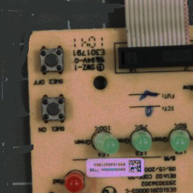
\includegraphics[width=1\textwidth]{images/guided/resize_circuit.png}
    \end{subfigure}
    \hfill
    \begin{subfigure}[t]{0.19\textwidth}
        \centering
        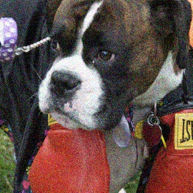
\includegraphics[width=1\textwidth]{images/guided/resize_dog.png}
    \end{subfigure}
    \hfill
    \begin{subfigure}[t]{0.19\textwidth}
        \centering
        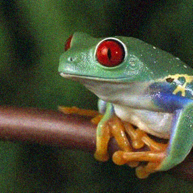
\includegraphics[width=1\textwidth]{images/guided/resize_frog.png}
    \end{subfigure}
    \hfill
    \begin{subfigure}[t]{0.19\textwidth}
        \centering
        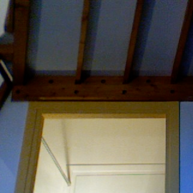
\includegraphics[width=1\textwidth]{images/guided/resize_room.png}
    \end{subfigure}
    \hfill
    \begin{subfigure}[t]{0.19\textwidth}
        \centering
        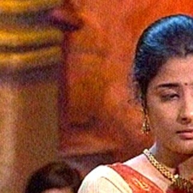
\includegraphics[width=1\textwidth]{images/guided/resize_singer.png}
    \end{subfigure}
    \hfill
    \begin{subfigure}[t]{0.19\textwidth}
        \centering
        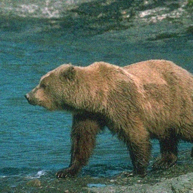
\includegraphics[width=1\textwidth]{images/guided/resize_bears.png}
    \end{subfigure}
    \hfill
    \begin{subfigure}[t]{0.19\textwidth}
        \centering
        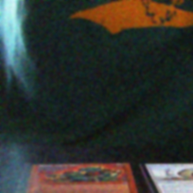
\includegraphics[width=1\textwidth]{images/guided/resize_cards.png}
    \end{subfigure}
    \hfill
    \begin{subfigure}[t]{0.19\textwidth}
        \centering
        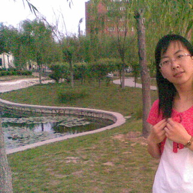
\includegraphics[width=1\textwidth]{images/guided/resize_girl.png}
    \end{subfigure}
    \hfill
    \begin{subfigure}[t]{0.19\textwidth}
        \centering
        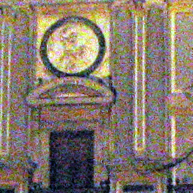
\includegraphics[width=1\textwidth]{images/guided/resize_palace.png}
    \end{subfigure}
    \hfill
    \begin{subfigure}[t]{0.19\textwidth}
        \centering
        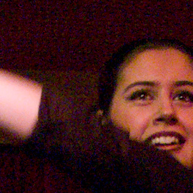
\includegraphics[width=1\textwidth]{images/guided/resize_woman.png}
    \end{subfigure}
    \caption{Some samples cropped from real noisy images of Dataset 1 \cite{ncwebsite}.}
    \label{fig3-3}
\end{figure}

\begin{figure}
    \centering
    \begin{subfigure}[t]{0.19\textwidth}
        \centering
        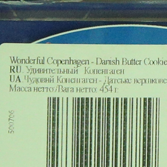
\includegraphics[width=1\textwidth]{images/guided/resize_CC_Noisy_Canon_EOS_5D_Mark3_ISO_3200_C1_52.png}
    \end{subfigure}
    \hfill
    \begin{subfigure}[t]{0.19\textwidth}
        \centering
        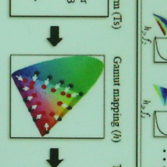
\includegraphics[width=1\textwidth]{images/guided/resize_CC_Noisy_Canon_EOS_5D_Mark3_ISO_3200_C2_44.png}
    \end{subfigure}
    \hfill
    \begin{subfigure}[t]{0.19\textwidth}
        \centering
        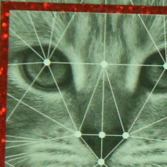
\includegraphics[width=1\textwidth]{images/guided/resize_CC_Noisy_Canon_EOS_5D_Mark3_ISO_3200_C3_26.png}
    \end{subfigure}
    \hfill
    \begin{subfigure}[t]{0.19\textwidth}
        \centering
        
\includegraphics[width=1\textwidth]{images/guided/resize_CC_Noisy_Canon_EOS_5D_Mark3_ISO_3200_C3_73.png}
    \end{subfigure}
    \hfill
    \begin{subfigure}[t]{0.19\textwidth}
        \centering
        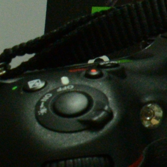
\includegraphics[width=1\textwidth]{images/guided/resize_CC_Noisy_Nikon_D600_ISO_3200_C2_67.png}
    \end{subfigure}
    \hfill
    \begin{subfigure}[t]{0.19\textwidth}
        \centering
        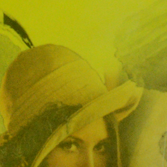
\includegraphics[width=1\textwidth]{images/guided/resize_CC_Noisy_Nikon_D800_ISO_1600_B2_80.png}
    \end{subfigure}
    \hfill
    \begin{subfigure}[t]{0.19\textwidth}
        \centering
        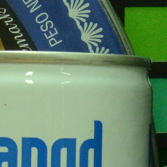
\includegraphics[width=1\textwidth]{images/guided/resize_CC_Noisy_Nikon_D800_ISO_1600_B3_82.png}
    \end{subfigure}
    \hfill
    \begin{subfigure}[t]{0.19\textwidth}
        \centering
        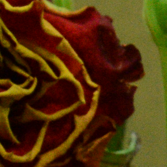
\includegraphics[width=1\textwidth]{images/guided/resize_CC_Noisy_Nikon_D800_ISO_3200_A4_51.png}
    \end{subfigure}
    \hfill
    \begin{subfigure}[t]{0.19\textwidth}
        \centering
        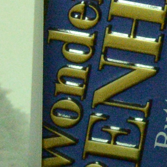
\includegraphics[width=1\textwidth]{images/guided/resize_CC_Noisy_Nikon_D800_ISO_6400_B3_95.png}
    \end{subfigure}
    \hfill
    \begin{subfigure}[t]{0.19\textwidth}
        \centering
        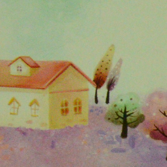
\includegraphics[width=1\textwidth]{images/guided/resize_CC_Noisy_Nikon_D800_ISO_3200_A2_80.png}
    \end{subfigure}
    \caption{Some samples cropped from real noisy images of Dataset 2 \cite{crosschannel2016}.}
    \label{fig3-4}
\end{figure}

\begin{figure}
    \centering
    \begin{subfigure}[t]{0.19\textwidth}
        \centering
        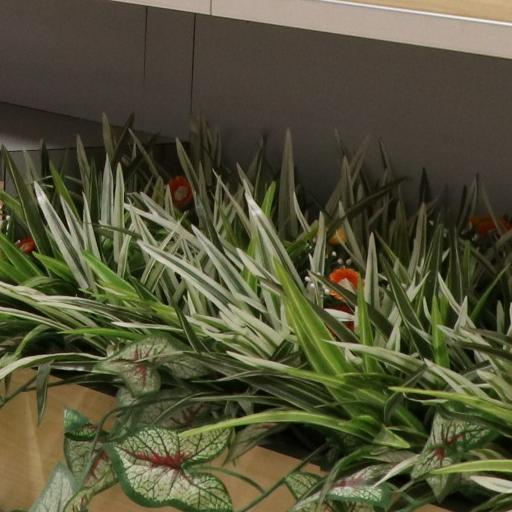
\includegraphics[width=1\textwidth]{images/guided/Canon_80D_ISO800_IMG_9916_part6.JPG}
    \end{subfigure}
    \hfill
    \begin{subfigure}[t]{0.19\textwidth}
        \centering
        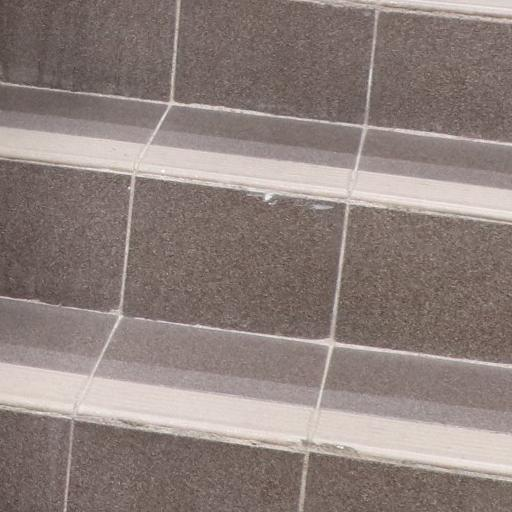
\includegraphics[width=1\textwidth]{images/guided/Canon_80D_ISO1600_IMG_1056_part2.JPG}
    \end{subfigure}
    \hfill
    \begin{subfigure}[t]{0.19\textwidth}
        \centering
        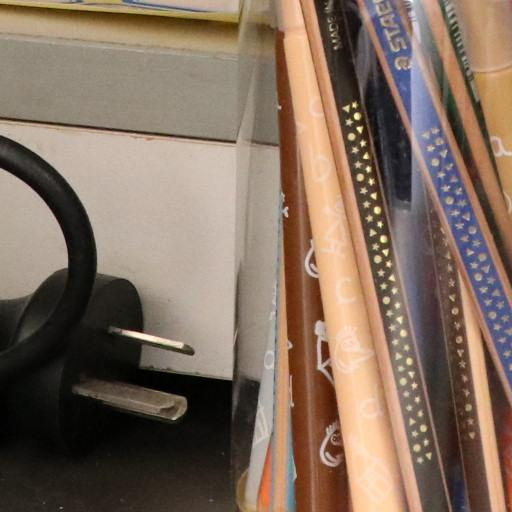
\includegraphics[width=1\textwidth]{images/guided/Canon_80D_ISO3200_IMG_8701_part8.JPG}
    \end{subfigure}
    \hfill
    \begin{subfigure}[t]{0.19\textwidth}
        \centering
        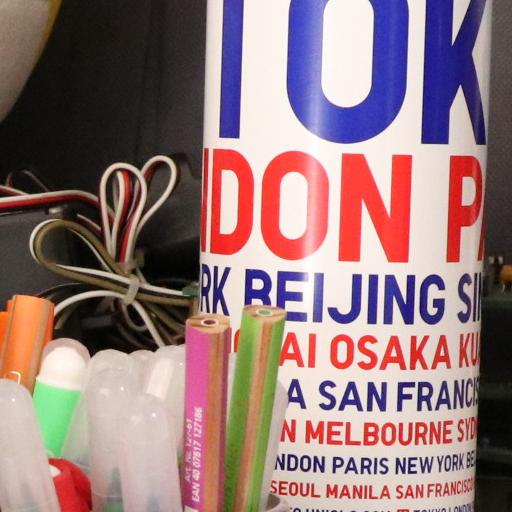
\includegraphics[width=1\textwidth]{images/guided/Canon_80D_ISO3200_IMG_8793_part10.JPG}
    \end{subfigure}
    \hfill
    \begin{subfigure}[t]{0.19\textwidth}
        \centering
        
\includegraphics[width=1\textwidth]{images/guided/Canon_80D_ISO3200_IMG_9133_part4.JPG}
    \end{subfigure}
    \hfill
    \begin{subfigure}[t]{0.19\textwidth}
        \centering
        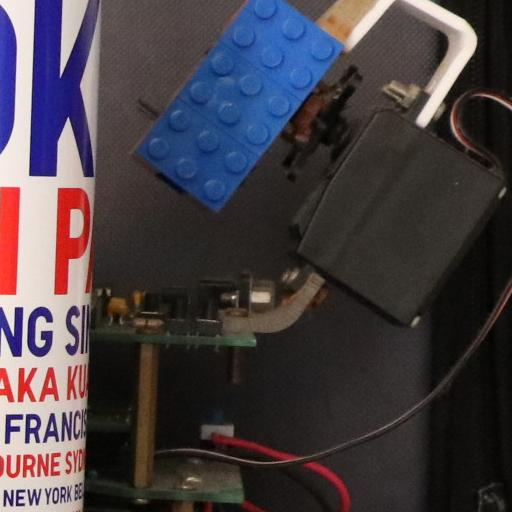
\includegraphics[width=1\textwidth]{images/guided/Canon_80D_ISO3200_IMG_9333_part6.JPG}
    \end{subfigure}
    \hfill
    \begin{subfigure}[t]{0.19\textwidth}
        \centering
        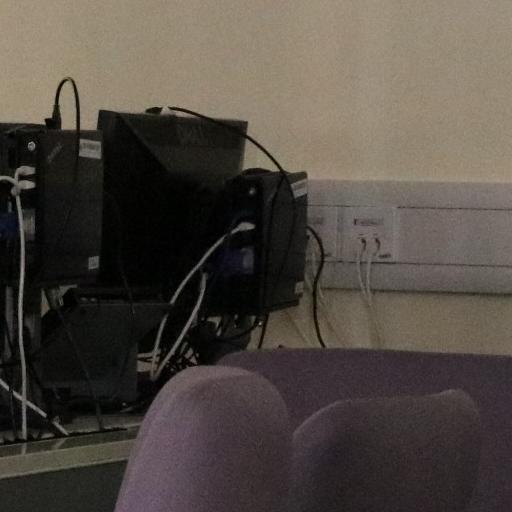
\includegraphics[width=1\textwidth]{images/guided/Canon_80D_ISO6400_IMG_0360_part2.JPG}
    \end{subfigure}
    \hfill
    \begin{subfigure}[t]{0.19\textwidth}
        \centering
        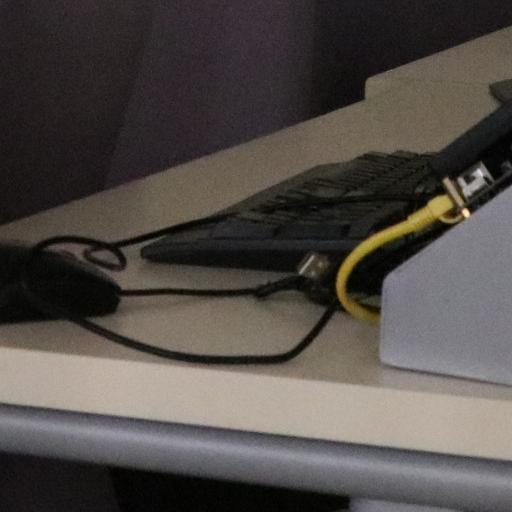
\includegraphics[width=1\textwidth]{images/guided/Canon_80D_ISO6400_IMG_0985_part5.JPG}
    \end{subfigure}
    \hfill
    \begin{subfigure}[t]{0.19\textwidth}
        \centering
        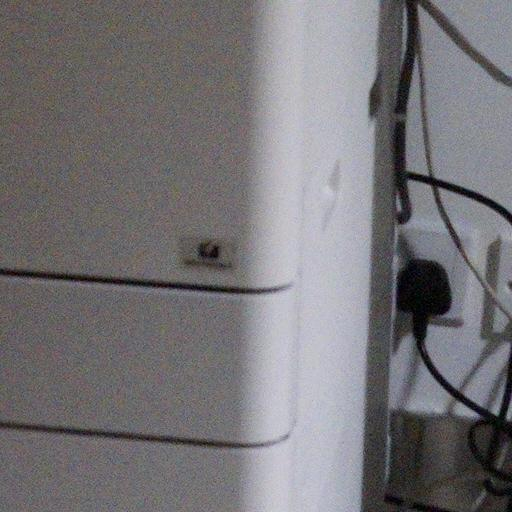
\includegraphics[width=1\textwidth]{images/guided/SONY_A7II_ISO12800_DSC02078_part1.JPG}
    \end{subfigure}
    \hfill
    \begin{subfigure}[t]{0.19\textwidth}
        \centering
        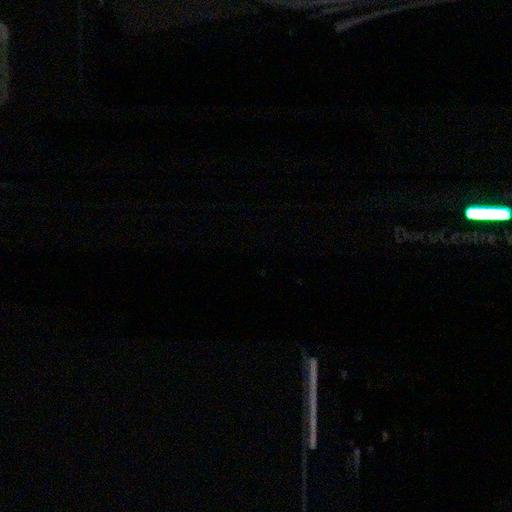
\includegraphics[width=1\textwidth]{images/guided/SONY_A7II_ISO12800_DSC02383_part8.JPG}
    \end{subfigure}
    \caption{Some samples cropped from our dataset (Dataset 3).}
    \label{fig3-5}
\end{figure}


\begin{figure}
    \centering
    \begin{subfigure}[t]{0.19\textwidth}
        \centering
        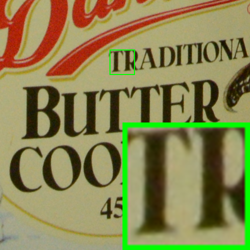
\includegraphics[width=1\textwidth]{images/guided/resize_br_Noisy_CC_Noisy_Nikon_D600_ISO_3200_C1_96.png}
		\caption{Noisy 35.89}
    \end{subfigure}
    \hfill
    \begin{subfigure}[t]{0.19\textwidth}
        \centering
        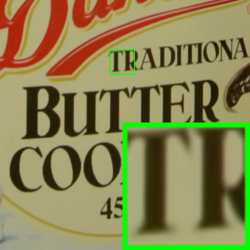
\includegraphics[width=1\textwidth]{images/guided/resize_br_Offline_CC_Noisy_Nikon_D600_ISO_3200_C1_96.png}
		\caption{External 39.05}
    \end{subfigure}
    \hfill
    \begin{subfigure}[t]{0.19\textwidth}
        \centering
        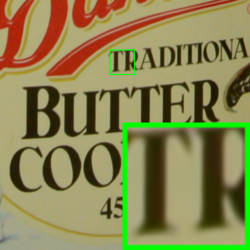
\includegraphics[width=1\textwidth]{images/guided/resize_br_Online_CC_Noisy_Nikon_D600_ISO_3200_C1_96.png}
\caption{Internal 38.75}
    \end{subfigure}
    \hfill
    \begin{subfigure}[t]{0.19\textwidth}
        \centering
        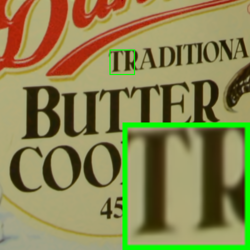
\includegraphics[width=1\textwidth]{images/guided/resize_br_Guided_CC_Noisy_Nikon_D600_ISO_3200_C1_96.png}
\caption{ Guided Internal \textbf{39.39}}
    \end{subfigure}
    \hfill
    \begin{subfigure}[t]{0.19\textwidth}
        \centering
        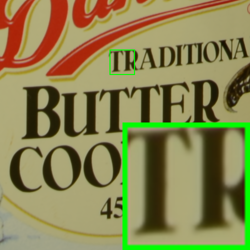
\includegraphics[width=1\textwidth]{images/guided/resize_br_Mean_CC_Noisy_Nikon_D600_ISO_3200_C1_96.png}
\caption{Mean Image}
    \end{subfigure}
    \caption{Denoised images and PSNR(dB) results of a region cropped from the real noisy image ``Nikon D600 ISO 3200 C1'' \cite{crosschannel2016} by different methods. The images are better to be zoomed in on screen.}
    \label{fig3-6}
\end{figure}


\begin{figure}
    \centering
    \begin{subfigure}[t]{0.19\textwidth}
        \centering
        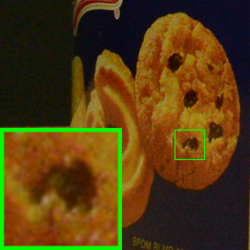
\includegraphics[width=1\textwidth]{images/guided/resize_br_Noisy_CC_Noisy_Nikon_D600_ISO_3200_C1_94b.png}
		\caption{Noisy 33.77}
    \end{subfigure}
    \hfill
    \begin{subfigure}[t]{0.19\textwidth}
        \centering
        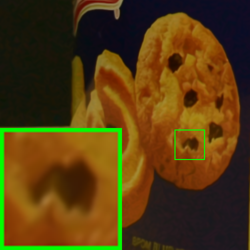
\includegraphics[width=1\textwidth]{images/guided/resize_br_Offline_CC_Noisy_Nikon_D600_ISO_3200_C1_94b.png}
		\caption{External 36.97}
    \end{subfigure}
    \hfill
    \begin{subfigure}[t]{0.19\textwidth}
        \centering
        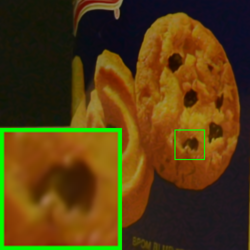
\includegraphics[width=1\textwidth]{images/guided/resize_br_Online_CC_Noisy_Nikon_D600_ISO_3200_C1_94b.png}
\caption{Internal 37.40}
    \end{subfigure}
    \hfill
    \begin{subfigure}[t]{0.19\textwidth}
        \centering
        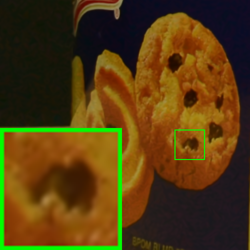
\includegraphics[width=1\textwidth]{images/guided/resize_br_Guided_CC_Noisy_Nikon_D600_ISO_3200_C1_94b.png}
\caption{ Guided Internal \textbf{38.01}}
    \end{subfigure}
    \hfill
    \begin{subfigure}[t]{0.19\textwidth}
        \centering
        \includegraphics[width=1\textwidth]{images/guided/resize_br_Mean_CC_Noisy_Nikon_D600_ISO_3200_C1_94b.png}
\caption{Mean Image}
    \end{subfigure}
    \caption{Denoised images and PSNR(dB) results of a region cropped from the real noisy image ``Nikon D600 ISO 3200 C1'' \cite{crosschannel2016} by different methods. The images are better to be zoomed in on screen.}
    \label{fig3-7}
\end{figure}


\subsection{Comparison among external, internal and guided internal priors}

To demonstrate the advantages of external prior guided internal prior learning, we perform real noisy image denoising by using external priors only (denoted by ``External''), internal priors only (denoted by ``Internal''), and the proposed guided internal priors (denoted by ``Guided Internal''), respectively.\ For the ``External'' method, we utilize the full external dictionaries (i.e., $r=108$ in Eq.\ (\ref{equ3-5})) for denoising.\ For the ``Internal'' method, the overall framework is similar to the method of \cite{ncsr}.\ A GMM model (with $K = 32$ Gaussians) is directly learned from the PGs extracted from the given noisy image without using any external data, and then the internal orthogonal dictionaries are obtained via Eq.\ (\ref{equ3-2}) to perform denoising.\ All parameters of the ``External'' and ``Internal'' methods are tuned to achieve their best performance. 

We compare the three methods on the 60 cropped images from \cite{crosschannel2016}.\ The average PSNR and run time are listed in Table \ref{tab1}.\ The best results are highlighted in bold.\ It can be seen that ``Guided Internal'' method achieves better PSNR than both ``External'' and ``Internal'' methods. In addition, the ``Internal'' method is very slow because it involves online GMM learning, while the ``Guided Internal'' method is only a little slower than the ``External'' method.\ Figs. \ref{fig3-6} and \ref{fig3-7} show the denoised images of two noisy images by the three methods.\ One can see that the  ``External'' method is good at recovering large-scale structures (see Fig. \ref{fig3-6}) while the ``Internal'' method is good at recovering fine-scale textures (see Fig. \ref{fig3-7}).\ By utilizing external priors to guide the internal prior learning, our proposed method can effectively recover both the large-scale structures and fine-scale textures. 

%------------------------------------------------------------------------------------
\begin{figure}
    \centering
    \begin{subfigure}[t]{0.19\textwidth}
        \centering
        \includegraphics[width=1\textwidth]{images/guided/resize_br_Noisy_dog.png}
		\caption{Noisy}
    \end{subfigure}
    \hfill
    \begin{subfigure}[t]{0.19\textwidth}
        \centering
        \includegraphics[width=1\textwidth]{images/guided/resize_br_BM3DPoisson_dog.png}
		\caption{GAT-BM3D}
    \end{subfigure}
    \hfill
    \begin{subfigure}[t]{0.19\textwidth}
        \centering
        \includegraphics[width=1\textwidth]{images/guided/resize_br_BM3D_dog.png}
\caption{CBM3D}
    \end{subfigure}
    \hfill
    \begin{subfigure}[t]{0.19\textwidth}
        \centering
        \includegraphics[width=1\textwidth]{images/guided/resize_br_WNNM_dog.png}
\caption{WNNM}
    \end{subfigure}
    \hfill
    \begin{subfigure}[t]{0.19\textwidth}
        \centering
        \includegraphics[width=1\textwidth]{images/guided/resize_br_CSF_dog.png}
\caption{CSF}
    \end{subfigure}
\hfill
    \begin{subfigure}[t]{0.19\textwidth}
        \centering
        \includegraphics[width=1\textwidth]{images/guided/resize_br_TRD_dog.png}
		\caption{TNRD}
    \end{subfigure}
    \hfill
    \begin{subfigure}[t]{0.19\textwidth}
        \centering
        \includegraphics[width=1\textwidth]{images/guided/resize_br_DnCNN_dog.png}
		\caption{DnCNN}
    \end{subfigure}
    \hfill
    \begin{subfigure}[t]{0.19\textwidth}
        \centering
        \includegraphics[width=1\textwidth]{images/guided/resize_br_NI_dog.png}
\caption{NI}
    \end{subfigure}
    \hfill
    \begin{subfigure}[t]{0.19\textwidth}
        \centering
        \includegraphics[width=1\textwidth]{images/guided/resize_br_NC_dog.png}
\caption{NC}
    \end{subfigure}
    \hfill
    \begin{subfigure}[t]{0.19\textwidth}
        \centering
        \includegraphics[width=1\textwidth]{images/guided/resize_br_Guided_dog.png}
\caption{Ours}
    \end{subfigure}
    \caption{Denoised images of the real noisy image ``Dog'' \cite{ncwebsite} by different methods. The images are better to be zoomed in on screen.}
    \label{fig3-8}
\end{figure}

\begin{figure}
    \centering
    \begin{subfigure}[t]{0.19\textwidth}
        \centering
        \includegraphics[width=1\textwidth]{images/guided/nc/resize_br_Noisy_frog.png}
		\caption{Noisy}
    \end{subfigure}
    \hfill
    \begin{subfigure}[t]{0.19\textwidth}
        \centering
        \includegraphics[width=1\textwidth]{images/guided/nc/resize_br_BM3DPoisson_frog.png}
		\caption{GAT-BM3D}
    \end{subfigure}
    \hfill
    \begin{subfigure}[t]{0.19\textwidth}
        \centering
        \includegraphics[width=1\textwidth]{images/guided/nc/resize_br_CBM3D_frog.png}
\caption{CBM3D}
    \end{subfigure}
    \hfill
    \begin{subfigure}[t]{0.19\textwidth}
        \centering
        \includegraphics[width=1\textwidth]{images/guided/nc/resize_br_WNNM_frog.png}
\caption{WNNM}
    \end{subfigure}
    \hfill
    \begin{subfigure}[t]{0.19\textwidth}
        \centering
        \includegraphics[width=1\textwidth]{images/guided/nc/resize_br_CSF_frog.png}
\caption{CSF}
    \end{subfigure}
\hfill
    \begin{subfigure}[t]{0.19\textwidth}
        \centering
        \includegraphics[width=1\textwidth]{images/guided/nc/resize_br_TRD_frog.png}
		\caption{TNRD}
    \end{subfigure}
    \hfill
    \begin{subfigure}[t]{0.19\textwidth}
        \centering
        \includegraphics[width=1\textwidth]{images/guided/nc/resize_br_DnCNN_frog.png}
		\caption{DnCNN}
    \end{subfigure}
    \hfill
    \begin{subfigure}[t]{0.19\textwidth}
        \centering
        \includegraphics[width=1\textwidth]{images/guided/nc/resize_br_NI_frog.png}
\caption{NI}
    \end{subfigure}
    \hfill
    \begin{subfigure}[t]{0.19\textwidth}
        \centering
        \includegraphics[width=1\textwidth]{images/guided/nc/resize_br_NC_frog.png}
\caption{NC}
    \end{subfigure}
    \hfill
    \begin{subfigure}[t]{0.19\textwidth}
        \centering
        \includegraphics[width=1\textwidth]{images/guided/nc/resize_br_Guided_frog.png}
\caption{Ours}
    \end{subfigure}
    \caption{Denoised images of the real noisy image ``Frog'' \cite{ncwebsite} by different methods. The images are better to be zoomed in on screen.}
    \label{fig3-9}
\end{figure}

\begin{figure}
    \centering
    \begin{subfigure}[t]{0.19\textwidth}
        \centering
        \includegraphics[width=1\textwidth]{images/guided/nc/resize_br_Noisy_circuit.png}
		\caption{Noisy}
    \end{subfigure}
    \hfill
    \begin{subfigure}[t]{0.19\textwidth}
        \centering
        \includegraphics[width=1\textwidth]{images/guided/nc/resize_br_BM3DPoisson_circuit.png}
		\caption{GAT-BM3D}
    \end{subfigure}
    \hfill
    \begin{subfigure}[t]{0.19\textwidth}
        \centering
        \includegraphics[width=1\textwidth]{images/guided/nc/resize_br_CBM3D_circuit.png}
\caption{CBM3D}
    \end{subfigure}
    \hfill
    \begin{subfigure}[t]{0.19\textwidth}
        \centering
        \includegraphics[width=1\textwidth]{images/guided/nc/resize_br_WNNM_circuit.png}
\caption{WNNM}
    \end{subfigure}
    \hfill
    \begin{subfigure}[t]{0.19\textwidth}
        \centering
        \includegraphics[width=1\textwidth]{images/guided/nc/resize_br_CSF_circuit.png}
\caption{CSF}
    \end{subfigure}
\hfill
    \begin{subfigure}[t]{0.19\textwidth}
        \centering
        \includegraphics[width=1\textwidth]{images/guided/nc/resize_br_TRD_circuit.png}
		\caption{TNRD}
    \end{subfigure}
    \hfill
    \begin{subfigure}[t]{0.19\textwidth}
        \centering
        \includegraphics[width=1\textwidth]{images/guided/nc/resize_br_DnCNN_circuit.png}
		\caption{DnCNN}
    \end{subfigure}
    \hfill
    \begin{subfigure}[t]{0.19\textwidth}
        \centering
        \includegraphics[width=1\textwidth]{images/guided/nc/resize_br_NI_circuit.png}
\caption{NI}
    \end{subfigure}
    \hfill
    \begin{subfigure}[t]{0.19\textwidth}
        \centering
        \includegraphics[width=1\textwidth]{images/guided/nc/resize_br_NC_circuit.png}
\caption{NC}
    \end{subfigure}
    \hfill
    \begin{subfigure}[t]{0.19\textwidth}
        \centering
        \includegraphics[width=1\textwidth]{images/guided/nc/resize_br_Guided_circuit.png}
\caption{Ours}
    \end{subfigure}
    \caption{Denoised images of the real noisy image ``Circuit'' \cite{ncwebsite} by different methods. The images are better to be zoomed in on screen.}
    \label{fig3-10}
\end{figure}

\subsection{Comparison with State-of-the-Art Denoising Methods}

\textbf{Comparison methods}.
We compare the proposed method with state-of-the-art image denoising methods, including GAT-BM3D \cite{makitalo2013optimal}, CBM3D \cite{cbm3d}, WNNM \cite{wnnm}, MLP \cite{mlp}, DnCNN \cite{dncnn}, CSF \cite{csf}, TNRD \cite{chen2015learning}, Noise Clinic (NC) \cite{noiseclinic,ncwebsite}, Cross-Channel (CC) \cite{crosschannel2016}, and Neat Image (NI) \cite{neatimage}.\ Among these methods, GAT-BM3D \cite{makitalo2013optimal} is a state-of-the-art Poisson noise reduction method.\ The method CBM3D \cite{cbm3d} is a state-of-the-art method for color image denoising and the noise on color images is assumed to be additive white Gaussian.\ The methods of WNNM, MLP, DnCNN, CSF, and TNRD are state-of-the-art Gaussian noise removal methods for grayscale images, and we apply them to each channel of color images for denoising. NC is a blind image denoising method, and NI is a set of commercial software for image denoising, which has been embedded into Photoshop and Corel PaintShop. The code of CC is not released but its results on the 15 cropped images are available at \cite{crosschannel2016}. Therefore, we only compare with it on the 15 cropped images in dataset 2 from \cite{crosschannel2016}. 

\textbf{Noise level of comparison methods.} 
For the CBM3D method, the standard deviation of noise on color images should be given as a parameter.\ For methods of WNNM, MLP, CSF, and TNRD, the noise level in each color channel should be input. For the DnCNN method, it is trained to deal with noise in a range of levels $0\sim55$.\ We retrain the models of discriminative denoising methods MLP, CSF, and TNRD (using the released codes by the authors) at different noise levels from $\sigma=5$ to $\sigma=50$ with a gap of $5$.\ The denoising is performed by processing each channel with the model trained at the same (or nearest) noise level.\ The noise levels ($\sigma_{r}, \sigma_{g}, \sigma_{b}$) in R, G ,B channels are assumed to be Gaussian and can be estimated via some noise estimation methods \cite{noiselevel,Chen2015ICCV}.\ In this paper, we employ the method \cite{Chen2015ICCV} to estimate the noise level for each color channel.

\begin{table}\vspace{-4mm}
\caption{Average PSNR (dB) and Run Time (seconds) of the ``External'', ``Internal'', and ``Guided Internal'' methods on 60 real noisy images (of size $500\times500\times3$) cropped from \cite{crosschannel2016}.}
\vspace{-4mm}
\label{tab3-1}
\begin{center}
\renewcommand\arraystretch{1}
\begin{tabular}{|c||c|c|c|c|}
\hline
 & \small\textbf{Noisy} &\small \textbf{External} & \small\textbf{Internal} & \small\textbf{Guided Internal}  
\\
\hline
PSNR & 34.51 & 38.21 & 38.07 & \textbf{38.75} 
\\
\hline
Time & | &  \textbf{21.19}  & 312.67 & 22.26
\\
\hline
\end{tabular}
\end{center}
\vspace{-3mm}
\end{table}

\textbf{Results on dataset 1.}
Since there is no ``ground truth'' for the real noisy images in  dataset 1 \cite{ncwebsite}, we only compare the visual quality of the denoised images by different methods. (Note that method CC \cite{crosschannel2016} is not compared since its code is not available. The result of MLP is not shown here due to the limit of space.) Fig. \ref{fig3-8} show the denoised images of ``Dog''. It can be seen that CBM3D and WNNM tend to over-smooth much the image while remaining some noise caused color artifacts.\ DnCNN and TNRD are likely to remain many noise-caused color artifacts across the whole image. These results demonstrate that the methods designed with Gaussian noise model are not effective for real noise removal.\ Though NC and NI methods are specifically developed for real noisy images, their performance on noise removal is not very satisfactory.\ In comparison, our proposed method recovers much better the structures and textures (such as the eye area in ``Dog'') than the other competing methods.\ More visual comparisons can be found in Figures \ref{fig3-9} and \ref{fig3-10}.


\begin{table}\vspace{-4mm}
\scriptsize
\begin{adjustwidth}{-2cm}{}
\caption{PSNR(dB) results of different methods on 15 cropped real noisy images used in \cite{crosschannel2016}.}
\vspace{-4mm}
\label{tab3-2}
\begin{center}
\renewcommand\arraystretch{1}
\begin{tabular}{|c||c|c|c|c|c|c|c|c|c|c|c|}
\hline
Camera Settings
&\textbf{GAT-BM3D}
&\textbf{CBM3D}
&\textbf{WNNM}
&\textbf{MLP}
&\textbf{CSF}
&\textbf{TNRD}
&\textbf{DnCNN}
& \textbf{NI}
&\textbf{NC}
&\textbf{CC} 
&\textbf{Ours} 
\\
\hline
\multirow{3}{*}{\small{Canon 5D Mark III}} 
& 31.23 & 39.76 & 37.51 & 39.00 & 35.68 & 39.51 & 37.26 & 37.68 & 38.76 & 38.37 & \textbf{40.50}
\\ 
\cdashline{2-12} 
\multirow{3}{*}{ISO = 3200}   
& 30.55 & 36.40 & 33.86 & 36.34 & 34.03 & 36.47 & 34.13 & 34.87 & 35.69 & 35.37 & \textbf{37.05}
\\ 
\cdashline{2-12}    
& 27.74 & 36.37 & 31.43 & 36.33 & 32.63 & \textbf{36.45} & 34.09 & 34.77 & 35.54 & 34.91 & 36.11 
\\
\hline
\multirow{3}{*}{Nikon D600} 
& 28.55 & 34.18 & 33.46 & 34.70 & 31.78 & 34.79 & 33.62 & 34.12 & \textbf{35.57} & 34.98 & 34.88
\\ 
\cdashline{2-12} 
\multirow{3}{*}{ISO = 3200}   
& 32.01 & 35.07 & 36.09 & 36.20 & 35.16 & 36.37 & 34.48 & 35.36 & \textbf{36.70} & 35.95 & 36.31
\\ 
\cdashline{2-12}    
& 39.78 & 37.13 & 39.86 & 39.33 & 39.98 & 39.49 & 35.41 & 38.68 & 39.28 & \textbf{41.15} & 39.23
\\
\hline
\multirow{3}{*}{Nikon D800} 
& 32.24 & 36.81 & 36.35 & 37.95 & 34.84 & 38.11 & 35.79 & 37.34 & 38.01 & 37.99 & \textbf{38.40}
\\ 
\cdashline{2-12} 
\multirow{3}{*}{ISO = 1600}   
& 33.86 & 37.76 & 39.99 & 40.23 & 38.42 & 40.52 & 36.08 & 38.57 & 39.05 & 40.36 & \textbf{40.92}
\\ 
\cdashline{2-12}    
& 33.90 & 37.51 & 37.15 & 37.94 & 35.79 & 38.17 & 35.48 & 37.87 & 38.20 & 38.30 & \textbf{38.97}
\\
\hline
\multirow{3}{*}{Nikon D800} 
& 36.49 & 35.05 & 38.60 & 37.55 & 38.36 & 37.69 & 34.08 & 36.95 & 38.07 & \textbf{39.01} & 38.66
\\ 
\cdashline{2-12} 
\multirow{3}{*}{ISO = 3200}   
& 32.91 & 34.07 & 36.04 & 35.91 & 35.53 & 35.90 & 33.70 & 35.09 & 35.72 & 36.75 & \textbf{37.07}
\\ 
\cdashline{2-12}    
& \textbf{40.20} & 34.42 & 39.73 & 38.15 & 40.05 & 38.21 & 33.31 & 36.91 & 36.76 & 39.06 & 38.52
\\ 
\hline
\multirow{3}{*}{Nikon D800} 
& 29.84 & 31.13 & 33.29 & 32.69 & 34.08 & 32.81 & 29.83 & 31.28 & 33.49 & \textbf{34.61} & 33.76
\\ 
\cdashline{2-12} 
\multirow{3}{*}{ISO = 6400}   
& 27.94 & 31.22 & 31.16 & 32.33 & 32.13 & 32.33 & 30.55 & 31.38 & 32.79 & 33.21 & \textbf{33.43}
\\ 
\cdashline{2-12}    
& 29.15 & 30.97 & 31.98 & 32.29 & 31.52 & 32.29 & 30.09 & 31.40 & 32.86 & 33.22 & \textbf{33.58}
\\
\hline
Average
& 32.43 & 35.19 & 35.77 & 36.46 & 35.33 & 36.61 & 33.86 & 35.49 & 36.43 & 36.88 & \textbf{37.15}
\\
\hline
\end{tabular}
\end{center}
\vspace{-3mm}
\end{adjustwidth}
\end{table}


In this section, we provide more comparisons of the proposed method with the state-of-the-art denoising methods on the 15 cropped real noisy images used in \cite{crosschannel2016}.\ In this dataset, each scene was shot 500 times under the same camera and camera setting.\ The mean image of the 500 shots is roughly taken as the ``ground truth'', with which the PSNR and SSIM \cite{ssim} can be computed.\  The average SSIM results of GAT-BM3D \cite{makitalo2013optimal}, CBM3D \cite{bm3d}, WNNM \cite{wnnm}, MLP \cite{mlp}, CSF \cite{csf}, TNRD \cite{chen2015learning}, DnCNN \cite{dncnn}, NI \cite{neatimage}, NC \cite{noiseclinic,ncwebsite}, CC \cite{crosschannel2016}, and the proposed method are listed in Table \ref{tab3-1}. As can be seen from Figures \ref{fig3-3}-\ref{fig3-4}, our proposed method achieves better performance than the the competing methods.

\begin{table}[htpb]
\begin{adjustwidth}{-3cm}{}
\caption{SSIM \cite{ssim} results of different methods on 15 cropped real noisy images used in \cite{crosschannel2016}.}
\vspace{-3mm}
\label{tab3-3}
\scriptsize
\begin{center}
\renewcommand\arraystretch{1}
\begin{tabular}{|c||c|c|c|c|c|c|c|c|c|c|c|}
\hline
Camera Settings
&
\textbf{GAT-BM3D}
&
\textbf{CBM3D}
&
\textbf{WNNM}
&
\textbf{MLP}
&
\textbf{CSF}
&
\textbf{TNRD}
&
\textbf{DnCNN}
&
\textbf{NI}
& 
\textbf{NC}
& 
\textbf{CC} 
&
\textbf{Ours} 
\\
\hline
\multirow{3}{*}{\small{Canon 5D Mark III}} 
& 0.9126 & 0.9778 & 0.9673 & 0.9695 & 0.9434 & 0.9742 & 0.9389 & 0.9600 & 0.9689 & 0.9678 & \textbf{0.9813}
\\ 
\cdashline{2-11} 
\multirow{3}{*}{ISO = 3200}   
& 0.8427 & 0.9552 & 0.9210 & 0.9458 & 0.9011 & 0.9491 & 0.8989 & 0.9308 & 0.9427 & 0.9359 & \textbf{0.9572}
\\ 
\cdashline{2-11}    
& 0.8017 & \textbf{0.9660} & 0.9110 & 0.9599 & 0.9037 & 0.9617 & 0.9182 & 0.9463 & 0.9476 & 0.9478 &  0.9643
\\
\hline
\multirow{3}{*}{Nikon D600} 
& 0.7845 & 0.9330 & 0.9281 & 0.9481 & 0.8792 & 0.9494 & 0.9123 & 0.9413 & 0.9497 & 0.9484 &  \textbf{0.9535}
\\ 
\cdashline{2-11} 
\multirow{3}{*}{ISO = 3200}   
& 0.9028 & 0.9168 & 0.9432 & 0.9469 & 0.9261 & \textbf{0.9499} & 0.8932 & 0.9251 & 0.9398 & 0.9293 &  0.9461
\\ 
\cdashline{2-11}    
& \textbf{0.9806} & 0.9313 & 0.9737 & 0.9726 & 0.9763 & 0.9742 & 0.8708 & 0.9481 & 0.9588 & 0.9799 &  0.9683
\\
\hline
\multirow{3}{*}{Nikon D800} 
& 0.8791 & 0.9339 & 0.9417 & 0.9543 & 0.9148 & 0.9572 & 0.9060 & 0.9506 & 0.9533 & 0.9575 &  \textbf{0.9620}
\\ 
\cdashline{2-11} 
\multirow{3}{*}{ISO = 1600}   
& 0.9534 & 0.9383 & 0.9748 & 0.9743 & 0.9674 & 0.9774 & 0.8943 & 0.9615 & 0.9591 & 0.9767 &  \textbf{0.9779}
\\ 
\cdashline{2-11}    
& 0.8795 & 0.9277 & 0.9311 & 0.9354 & 0.9035 & 0.9410 & 0.8735 & 0.9229 & 0.9406 & 0.9427 &  \textbf{0.9531}
\\
\hline
\multirow{3}{*}{Nikon D800} 
& 0.9526 & 0.8866 & \textbf{0.9656} & 0.9533 & 0.9654 & 0.9569 & 0.8463 & 0.9101 & 0.9466 & 0.9637 &  0.9613
\\ 
\cdashline{2-11} 
\multirow{3}{*}{ISO = 3200}   
& 0.9078 & 0.8928 & 0.9416 & 0.9381 & 0.9354 & 0.9394 & 0.8755 & 0.9194 & 0.9309 & 0.9477 &  \textbf{0.9521}
\\ 
\cdashline{2-11}    
& 0.9707 & 0.8430 & 0.9664 & 0.9548 & \textbf{0.9712} & 0.9576 & 0.7204 & 0.9001 & 0.9070 & 0.9544 &  0.9512
\\ 
\hline
\multirow{3}{*}{Nikon D800} 
& 0.8909 & 0.7952 & 0.9188 & 0.8914 & \textbf{0.9259} & 0.8966 & 0.7847 & 0.7781 & 0.9024 & 0.9206 &  0.8958
\\ 
\cdashline{2-11} 
\multirow{3}{*}{ISO = 6400}   
& 0.8328 & 0.8613 & 0.9050 & 0.9137 & 0.9127 & 0.9142 & 0.8259 & 0.8649 & 0.9141 & \textbf{0.9369} &  0.9238
\\ 
\cdashline{2-11}    
& 0.7773 & 0.8363 & 0.8818 & 0.8958 & 0.8494 & 0.8960 & 0.7936 & 0.8295 & 0.8847 & \textbf{0.9118} & 0.9089
\\
\hline
Average
& 0.8846 & 0.9063 & 0.9381 & 0.9436 & 0.9250 & 0.9463 & 0.8635 & 0.9126 & 0.9364 & 0.9481 & \textbf{0.9504}
\\
\hline
\end{tabular}
\end{center}
\end{adjustwidth}
\end{table}

\textbf{Results on dataset 2.}
As described in section 3.4.2, there is a mean image for each of the 11 scenes used in dataset 2 \cite{crosschannel2016}, and those mean images can be roughly taken as ``ground truth'' images for quantitative evaluation of denoising algorithms. We firstly perform quantitative comparison on the 15 cropped images used in \cite{crosschannel2016}. The PSNR results of GAT-BM3D, CBM3D, WNNM, MLP, CSF, TNRD, DnCNN, NC, NI and CC are listed in Table II (The results of CC are copied from the original paper \cite{crosschannel2016}). The best PSNR results of each image are highlighted in bold. One can see that on 8 out of the 15 images, our method achieves the best PSNR values. CC achieves the best PSNR on 3 of the 15 images. It should be noted that in the CC method, a specific model is trained for each camera and camera setting, while our method uses the same model for all images. On average, our proposed method has 0.27dB PSNR improvements over the second best method CC and much higher PSNR gains over other competing methods. The method GAT-BM3D does not work well on most images. This is because real world noise is much more complex than Poisson. 

Fig. \ref{fig3-11} shows the denoised images of one scene captured by Canon 5D Mark 3 at ISO = 3200. We can see that GAT-BM3D, CBM3D, WNNM, DnCNN, NC, NI and CC would either remain noise or generate artifacts, while TNRD over-smooths much the image. By using the external prior guided internal priors, our proposed method preserves edges and textures better than other methods, leading to visually pleasant outputs. More comparisons on visual quality and SSIM \cite{ssim} index can be found in the Figures \ref{fig3-12} and \ref{fig3-13}.

We then perform denoising experiments on the 60 images we cropped from \cite{crosschannel2016}. The average PSNR results are listed in Table III (CC is not compared since the code is not available). Again, our proposed method achieves much better PSNR results than the other methods. The improvements of our method over the second best method (TNRD) are 0.43dB on PSNR. Fig. \ref{fig3-14} shows the denoised images of one scene captured by Nikon D800 at ISO = 3200. We can see again that the proposed method obtain better visual quality than other competing methods. More comparisons on visual quality and SSIM can be found in the Figures \ref{fig3-15} and \ref{fig3-16}.

\textbf{Results on dataset 3.}
Similar to dataset 2 \cite{crosschannel2016}, there is a ``ground truth'' image for each of the 10 scenes used in our constructed dataset 3. We perform quantitative comparison on the 100 cropped images. The average PSNR results of competing methods are listed in Table IV. We can see that our proposed method achieves much better PSNR results than the other methods. The improvements of our method over the second best method (TNRD) is 0.16dB on PSNR. Fig. \ref{fig3-17} shows the denoised images of one scene captured by Canon 80D at ISO = 12800. We can see again that the proposed method removes the noise while maintains better details (such as the vertical black shadow area) than other competing methods. More comparisons on visual quality and SSIM can be found in the Figures \ref{fig3-18} and \ref{fig3-19}.

\textbf{Comparison on speed.}
Efficiency is an important aspect to evaluate the efficiency of algorithms. We compare the speed of all competing methods except for CC. All experiments are run under the Matlab2014b environment on a machine with Intel(R) Core(TM) i7-5930K CPU of 3.5GHz and 32GB RAM. The average running time (second) of the compared methods on the 100 real noisy images is shown in Table \ref{tab3-5}. The least average running time are highlighted in bold. One can easily see that the commercial software Neat Image (NI) is the fastest method with highly optimized code. For a $512\times512$ image, NI costs about 0.6 second. The other methods cost from 5.2 (TNRD) to 152.2 (WNNM) seconds, while the proposed method costs about 24.1 seconds. It should be noted that GAT-BM3D, CBM3D, TNRD, and NC are implemented with compiled C++ mex-function and with parallelization, while WNNM, MLP, CSF, DnCNN, and the proposed method are implemented purely in Matlab. 


\begin{figure}
    \centering
    \begin{subfigure}[t]{0.19\textwidth}
        \centering
        \includegraphics[width=1\textwidth]{images/guided/resize_br_Noisy_5dmark3_iso3200_1_real.png}
		\caption{Noisy 37.00}
    \end{subfigure}
    \hfill
    \begin{subfigure}[t]{0.19\textwidth}
        \centering
        \includegraphics[width=1\textwidth]{images/guided/resize_br_CBM3D_5dmark3_iso3200_1_real.png}
		\caption{CBM3D39.76}
    \end{subfigure}
    \hfill
    \begin{subfigure}[t]{0.19\textwidth}
        \centering
        \includegraphics[width=1\textwidth]{images/guided/resize_br_WNNM_5dmark3_iso3200_1_real.png}
\caption{WNNM 37.51}
    \end{subfigure}
    \hfill
    \begin{subfigure}[t]{0.19\textwidth}
        \centering
        \includegraphics[width=1\textwidth]{images/guided/resize_br_TRD_5dmark3_iso3200_1_real.png}
\caption{TNRD 39.51}
    \end{subfigure}
    \hfill
    \begin{subfigure}[t]{0.19\textwidth}
        \centering
        \includegraphics[width=1\textwidth]{images/guided/resize_br_DnCNN_5dmark3_iso3200_1_real.png}
\caption{DnCNN 37.26}
    \end{subfigure}
\hfill
    \begin{subfigure}[t]{0.19\textwidth}
        \centering
        \includegraphics[width=1\textwidth]{images/guided/resize_br_NI_5dmark3_iso3200_1_real.png}
		\caption{NI 37.68}
    \end{subfigure}
    \hfill
    \begin{subfigure}[t]{0.19\textwidth}
        \centering
        \includegraphics[width=1\textwidth]{images/guided/resize_br_NC_5dmark3_iso3200_1_real.png}
		\caption{NC 38.76}
    \end{subfigure}
    \hfill
    \begin{subfigure}[t]{0.19\textwidth}
        \centering
        \includegraphics[width=1\textwidth]{images/guided/resize_br_CCNoise_5dmark3_iso3200_1.png}
\caption{CC 38.37}
    \end{subfigure}
    \hfill
    \begin{subfigure}[t]{0.19\textwidth}
        \centering
        \includegraphics[width=1\textwidth]{images/guided/resize_br_Guided_5dmark3_iso3200_1.png}
\caption{Ours \textbf{40.50}}
    \end{subfigure}
    \hfill
    \begin{subfigure}[t]{0.19\textwidth}
        \centering
        \includegraphics[width=1\textwidth]{images/guided/resize_br_Mean_5dmark3_iso3200_1_real.png}
\caption{Mean Image}
    \end{subfigure}
    \caption{Denoised images and PSNR(dB) results of a region cropped from the real noisy image ``Canon 5D Mark 3 ISO 3200 1'' \cite{crosschannel2016} by different methods. The images are better to be zoomed in on screen.}
    \label{fig3-11}
\end{figure}


\begin{figure}
    \centering
    \begin{subfigure}[t]{0.19\textwidth}
        \centering
        \includegraphics[width=1\textwidth]{images/guided/cc15/resize_br_Noisy_5dmark3_iso3200_2_real.png}
		\caption{Noisy 33.88}
    \end{subfigure}
    \hfill
    \begin{subfigure}[t]{0.19\textwidth}
        \centering
        \includegraphics[width=1\textwidth]{images/guided/cc15/resize_br_CBM3D_5dmark3_iso3200_2_real.png}
		\caption{CBM3D 36.40}
    \end{subfigure}
    \hfill
    \begin{subfigure}[t]{0.19\textwidth}
        \centering
        \includegraphics[width=1\textwidth]{images/guided/cc15/resize_br_WNNM_5dmark3_iso3200_2_real.png}
\caption{WNNM 33.86}
    \end{subfigure}
    \hfill
    \begin{subfigure}[t]{0.19\textwidth}
        \centering
        \includegraphics[width=1\textwidth]{images/guided/cc15/resize_br_TRD_5dmark3_iso3200_2_real.png}
\caption{TNRD 36.47}
    \end{subfigure}
    \hfill
    \begin{subfigure}[t]{0.19\textwidth}
        \centering
        \includegraphics[width=1\textwidth]{images/guided/cc15/resize_br_DnCNN_5dmark3_iso3200_2_real.png}
\caption{DnCNN 34.13}
    \end{subfigure}
\hfill
    \begin{subfigure}[t]{0.19\textwidth}
        \centering
        \includegraphics[width=1\textwidth]{images/guided/cc15/resize_br_NI_5dmark3_iso3200_2_real.png}
		\caption{NI 34.87}
    \end{subfigure}
    \hfill
    \begin{subfigure}[t]{0.19\textwidth}
        \centering
        \includegraphics[width=1\textwidth]{images/guided/cc15/resize_br_NC_5dmark3_iso3200_2_real.png}
		\caption{NC 35.69}
    \end{subfigure}
    \hfill
    \begin{subfigure}[t]{0.19\textwidth}
        \centering
        \includegraphics[width=1\textwidth]{images/guided/cc15/resize_br_CCNoise_5dmark3_iso3200_2.png}
\caption{CC 35.37}
    \end{subfigure}
    \hfill
    \begin{subfigure}[t]{0.19\textwidth}
        \centering
        \includegraphics[width=1\textwidth]{images/guided/cc15/resize_br_Guided_5dmark3_iso3200_2_real.png}
\caption{Ours \textbf{37.05}}
    \end{subfigure}
    \hfill
    \begin{subfigure}[t]{0.19\textwidth}
        \centering
        \includegraphics[width=1\textwidth]{images/guided/cc15/resize_br_Mean_5dmark3_iso3200_2_real.png}
\caption{Mean Image}
    \end{subfigure}
    \caption{Denoised images and PSNR(dB) results of a region cropped from the real noisy image ``Canon 5D Mark 3 ISO 3200 2'' \cite{crosschannel2016} by different methods. The images are better to be zoomed in on screen.}
    \label{fig3-12}
\end{figure}

\begin{figure}
    \centering
    \begin{subfigure}[t]{0.19\textwidth}
        \centering
        \includegraphics[width=1\textwidth]{images/guided/cc15/resize_br_Noisy_d600_iso3200_2_real.png}
		\caption{Noisy 33.77}
    \end{subfigure}
    \hfill
    \begin{subfigure}[t]{0.19\textwidth}
        \centering
        \includegraphics[width=1\textwidth]{images/guided/cc15/resize_br_CBM3D_d600_iso3200_2_real.png}
		\caption{CBM3D 35.07}
    \end{subfigure}
    \hfill
    \begin{subfigure}[t]{0.19\textwidth}
        \centering
        \includegraphics[width=1\textwidth]{images/guided/cc15/resize_br_WNNM_d600_iso3200_2_real.png}
\caption{WNNM 36.09}
    \end{subfigure}
    \hfill
    \begin{subfigure}[t]{0.19\textwidth}
        \centering
        \includegraphics[width=1\textwidth]{images/guided/cc15/resize_br_TRD_d600_iso3200_2_real.png}
\caption{TNRD 36.37}
    \end{subfigure}
    \hfill
    \begin{subfigure}[t]{0.19\textwidth}
        \centering
        \includegraphics[width=1\textwidth]{images/guided/cc15/resize_br_DnCNN_d600_iso3200_2_real.png}
\caption{DnCNN 34.48}
    \end{subfigure}
\hfill
    \begin{subfigure}[t]{0.19\textwidth}
        \centering
        \includegraphics[width=1\textwidth]{images/guided/cc15/resize_br_NI_d600_iso3200_2_real.png}
		\caption{NI 35.36}
    \end{subfigure}
    \hfill
    \begin{subfigure}[t]{0.19\textwidth}
        \centering
        \includegraphics[width=1\textwidth]{images/guided/cc15/resize_br_NC_d600_iso3200_2_real.png}
		\caption{NC \textbf{36.70}}
    \end{subfigure}
    \hfill
    \begin{subfigure}[t]{0.19\textwidth}
        \centering
        \includegraphics[width=1\textwidth]{images/guided/cc15/resize_br_CCNoise_d600_iso3200_2.png}
\caption{CC 35.95}
    \end{subfigure}
    \hfill
    \begin{subfigure}[t]{0.19\textwidth}
        \centering
        \includegraphics[width=1\textwidth]{images/guided/cc15/resize_br_Guided_d600_iso3200_2_real.png}
\caption{Ours 36.31}
    \end{subfigure}
    \hfill
    \begin{subfigure}[t]{0.19\textwidth}
        \centering
        \includegraphics[width=1\textwidth]{images/guided/cc15/resize_br_Mean_d600_iso3200_2_real.png}
\caption{Mean Image}
    \end{subfigure}
    \caption{Denoised images and PSNR(dB) results of a region cropped from the real noisy image ``Nikon D600 ISO 3200 2'' \cite{crosschannel2016} by different methods. The images are better to be zoomed in on screen.}
    \label{fig3-13}
\end{figure}


\begin{table}
\begin{adjustwidth}{-1cm}{}
\scriptsize
\caption{Average PSNR(dB) results of different methods on 60 real noisy images cropped from \cite{crosschannel2016}.}
\vspace{-4mm}
\label{tab3-4}
\begin{center}
\renewcommand\arraystretch{1}
\begin{tabular}{|c||c|c|c|c|c|c|c|c|c|c|}
\hline
Methods
&\textbf{GAT-BM3D}
&\textbf{CBM3D}
&\textbf{WNNM}
&\textbf{MLP}
&\textbf{CSF} 
&\textbf{TNRD} 
&\textbf{DnCNN}
&\textbf{NI} 
&\textbf{NC} 
&\textbf{Ours} 
\\
\hline
PSNR  
& 34.33 & 36.34 & 37.67 & 38.13 & 37.40 & 38.32 & 34.99 & 36.53 & 37.57 & \textbf{38.75}
\\
\hline
\end{tabular}
\end{center}
\end{adjustwidth}
\end{table}

In this section, we provide more comparisons of the proposed method with the state-of-the-art denoising methods on the 60 real noisy images cropped from \cite{crosschannel2016}.\ In this dataset, each scene was shot 500 times under the same camera and camera setting.\ The mean image of the 500 shots is roughly taken as the ``ground truth'', with which the PSNR and SSIM can be computed.\ The average SSIM results of GAT-BM3D \cite{makitalo2013optimal}, CBM3D \cite{bm3d}, WNNM \cite{wnnm}, MLP \cite{mlp}, CSF \cite{csf}, TNRD \cite{chen2015learning}, DnCNN \cite{dncnn}, NI \cite{neatimage}, NC \cite{noiseclinic,ncwebsite}, and the proposed method are listed in Table \ref{tab3-4} (CC is not compared since the code of \cite{crosschannel2016} is not available).\ As can be seen from Figures \ref{fig3-5}-\ref{fig3-6}, our proposed method achieves better performance than the competing methods.

\begin{table}[htpb]
\begin{adjustwidth}{-1cm}{}
\scriptsize
\caption{Average SSIM \cite{ssim} results of different methods on 60 real noisy images cropped from \cite{crosschannel2016}.}
\label{tab3-5}
\begin{center}
\renewcommand\arraystretch{1}
\begin{tabular}{|c||c|c|c|c|c|c|c|c|c|c|}
\hline
Methods
&\textbf{GAT-BM3D}
&\textbf{CBM3D}
&\textbf{WNNM}
&\textbf{MLP}
&\textbf{CSF} 
&\textbf{TNRD} 
&\textbf{DnCNN}
&\textbf{NI} 
&\textbf{NC} 
&\textbf{Ours} 
\\
\hline
SSIM  
& 0.9331 & 0.9251 & 0.9633 & 0.9653 & 0.9598 & 0.9670 & 0.8873 & 0.9241 & 0.9514 & \textbf{0.9691}
\\
\hline
\end{tabular}
\end{center}
\end{adjustwidth}
\end{table}




\begin{table}
\begin{adjustwidth}{-2cm}{}
\scriptsize
\caption{Average PSNR(dB) results of different methods on 100 real noisy images cropped from our new dataset.}
\vspace{-4mm}
\label{tab3-6}
\begin{center}
\renewcommand\arraystretch{1}
\begin{tabular}{|c||c|c|c|c|c|c|c|c|c|c|}
\hline
Methods
&\textbf{GAT-BM3D}
&\textbf{CBM3D}
&\textbf{WNNM}
&\textbf{MLP}
&\textbf{CSF} 
&\textbf{TNRD} 
&\textbf{DnCNN}
&\textbf{NI} 
&\textbf{NC} 
&\textbf{Ours} 
\\
\hline
PSNR  
& 33.54 & 37.14 & 35.18 & 37.34 & 37.07 & 37.48 & 34.74 & 35.70 & 36.76 & \textbf{37.64}
\\
\hline
\end{tabular}
\end{center}
\end{adjustwidth}
\end{table}

In this section, we provide more comparisons of the proposed method with the state-of-the-art denoising methods on the 100 real noisy images cropped from the new dataset we constructed.\ In this dataset, each scene was shot 500 times under the same camera and camera setting.\ The mean image of the 500 shots is roughly taken as the ``ground truth'', with which the PSNR and SSIM can be computed.\ The average  SSIM results of GAT-BM3D \cite{makitalo2013optimal}, CBM3D \cite{bm3d}, WNNM \cite{wnnm}, MLP \cite{mlp}, CSF \cite{csf}, TNRD \cite{chen2015learning}, DnCNN \cite{dncnn}, NI \cite{neatimage}, NC \cite{noiseclinic,ncwebsite}, and the proposed method are listed in Table \ref{tab3-7} (CC is not compared since the code of \cite{crosschannel2016} is not available).\ As can be seen from Figure \ref{fig3-11}, our proposed method achieves better performance than the competing methods.


\begin{table}[htpb]
\begin{adjustwidth}{-1cm}{}
\scriptsize
\caption{Average SSIM \cite{ssim} results of different methods on 100 real noisy images cropped from our new dataset.}
\label{tab3-7}
\begin{center}
\renewcommand\arraystretch{1}
\begin{tabular}{|c||c|c|c|c|c|c|c|c|c|c|}
\hline
Methods
&\textbf{GAT-BM3D}
&\textbf{CBM3D}
&\textbf{WNNM}
&\textbf{MLP}
&\textbf{CSF} 
&\textbf{TNRD} 
&\textbf{DnCNN}
&\textbf{NI} 
&\textbf{NC} 
&\textbf{Ours} 
\\
\hline
SSIM  
& 0.8881 & 0.9494 & 0.9290 & 0.9453 & 0.9398 & 0.9486 & 0.8852 & 0.9190 & 0.9356 & \textbf{0.9529}
\\
\hline
\end{tabular}
\end{center}
\end{adjustwidth}
\end{table}



\begin{table}\vspace{-4mm}
\begin{adjustwidth}{-1cm}{}
\scriptsize
\caption{Average Speed (sec.) results of different methods on 100 real noisy images cropped from our new dataset.}
\vspace{-4mm}
\label{tab3-8}
\begin{center}
\renewcommand\arraystretch{1}
\begin{tabular}{|c||c|c|c|c|c|c|c|c|c|c|}
\hline
Methods
&\textbf{GAT-BM3D}
&\textbf{CBM3D}
&\textbf{WNNM}
&\textbf{MLP}
&\textbf{CSF} 
&\textbf{TNRD} 
&\textbf{DnCNN}
&\textbf{NI} 
&\textbf{NC} 
&\textbf{Ours} 
\\
\hline
Time  
& 11.1 & 6.9 & 152.2 & 17.1 & 19.5 & 5.2 & 79.5 & \textbf{0.6} & 15.6 & 24.1
\\
\hline
\end{tabular}
\end{center}
\end{adjustwidth}
\end{table}


%------------------------------------------------------------------------------------
\begin{figure}
    \centering
    \begin{subfigure}[t]{0.19\textwidth}
        \centering
        \includegraphics[width=1\textwidth]{images/guided/resize_br_Noisy_CC_Noisy_Nikon_D800_ISO_3200_A3_96.png}
		\caption{Noisy 33.60}
    \end{subfigure}
    \hfill
    \begin{subfigure}[t]{0.19\textwidth}
        \centering
        \includegraphics[width=1\textwidth]{images/guided/resize_br_CBM3D_CC_Noisy_Nikon_D800_ISO_3200_A3_96.png}
		\caption{CBM3D35.23}
    \end{subfigure}
    \hfill
    \begin{subfigure}[t]{0.19\textwidth}
        \centering
        \includegraphics[width=1\textwidth]{images/guided/resize_br_WNNM_CC_Noisy_Nikon_D800_ISO_3200_A3_96.png}
\caption{WNNM 36.50}
    \end{subfigure}
    \hfill
    \begin{subfigure}[t]{0.19\textwidth}
        \centering
        \includegraphics[width=1\textwidth]{images/guided/resize_br_CSF_CC_Noisy_Nikon_D800_ISO_3200_A3_96.png}
\caption{CSF 36.21}
    \end{subfigure}
    \hfill
    \begin{subfigure}[t]{0.19\textwidth}
        \centering
        \includegraphics[width=1\textwidth]{images/guided/resize_br_TRD_CC_Noisy_Nikon_D800_ISO_3200_A3_96.png}
\caption{TNRD 37.10}
    \end{subfigure}
\hfill
    \begin{subfigure}[t]{0.19\textwidth}
        \centering
        \includegraphics[width=1\textwidth]{images/guided/resize_br_DnCNN_CC_Noisy_Nikon_D800_ISO_3200_A3_96.png}
		\caption{DnCNN 34.43}
    \end{subfigure}
    \hfill
    \begin{subfigure}[t]{0.19\textwidth}
        \centering
        \includegraphics[width=1\textwidth]{images/guided/resize_br_NI_CC_Noisy_Nikon_D800_ISO_3200_A3_96.png}
		\caption{NI 35.02}
    \end{subfigure}
    \hfill
    \begin{subfigure}[t]{0.19\textwidth}
        \centering
        \includegraphics[width=1\textwidth]{images/guided/resize_br_NC_CC_Noisy_Nikon_D800_ISO_3200_A3_96.png}
\caption{NC 36.07}
    \end{subfigure}
    \hfill
    \begin{subfigure}[t]{0.19\textwidth}
        \centering
        \includegraphics[width=1\textwidth]{images/guided/resize_br_Guided_CC_Noisy_Nikon_D800_ISO_3200_A3_96.png}
\caption{Ours \textbf{37.50}}
    \end{subfigure}
    \hfill
    \begin{subfigure}[t]{0.19\textwidth}
        \centering
        \includegraphics[width=1\textwidth]{images/guided/resize_br_Mean_CC_Noisy_Nikon_D800_ISO_3200_A3_96.png}
\caption{Mean Image}
    \end{subfigure}
    \caption{Denoised images and PSNR(dB) results of a region cropped from the real noisy image ``Nikon D800 ISO 3200 A3'' \cite{crosschannel2016} by different methods. The images are better to be zoomed in on screen.}
    \label{fig3-14}
\end{figure}

\begin{figure}
    \centering
    \begin{subfigure}[t]{0.19\textwidth}
        \centering
        \includegraphics[width=1\textwidth]{images/guided/cc60/resize_br_Noisy_CC_Noisy_Nikon_D800_ISO_1600_B2_109.png}
		\caption{Noisy 35.21}
    \end{subfigure}
    \hfill
    \begin{subfigure}[t]{0.19\textwidth}
        \centering
        \includegraphics[width=1\textwidth]{images/guided/cc60/resize_br_CBM3D_CC_Noisy_Nikon_D800_ISO_1600_B2_109.png}
		\caption{CBM3D 37.71}
    \end{subfigure}
    \hfill
    \begin{subfigure}[t]{0.19\textwidth}
        \centering
        \includegraphics[width=1\textwidth]{images/guided/cc60/resize_br_WNNM_CC_Noisy_Nikon_D800_ISO_1600_B2_109.png}
\caption{WNNM 39.61}
    \end{subfigure}
    \hfill
    \begin{subfigure}[t]{0.19\textwidth}
        \centering
        \includegraphics[width=1\textwidth]{images/guided/cc60/resize_br_CSF_CC_Noisy_Nikon_D800_ISO_1600_B2_109.png}
\caption{CSF 38.14}
    \end{subfigure}
    \hfill
    \begin{subfigure}[t]{0.19\textwidth}
        \centering
        \includegraphics[width=1\textwidth]{images/guided/cc60/resize_br_TRD_CC_Noisy_Nikon_D800_ISO_1600_B2_109.png}
\caption{TNRD 39.04}
    \end{subfigure}
\hfill
    \begin{subfigure}[t]{0.19\textwidth}
        \centering
        \includegraphics[width=1\textwidth]{images/guided/cc60/resize_br_DnCNN_CC_Noisy_Nikon_D800_ISO_1600_B2_109.png}
		\caption{DnCNN 35.68}
    \end{subfigure}
    \hfill
    \begin{subfigure}[t]{0.19\textwidth}
        \centering
        \includegraphics[width=1\textwidth]{images/guided/cc60/resize_br_NI_CC_Noisy_Nikon_D800_ISO_1600_B2_109.png}
		\caption{NI 37.41}
    \end{subfigure}
    \hfill
    \begin{subfigure}[t]{0.19\textwidth}
        \centering
        \includegraphics[width=1\textwidth]{images/guided/cc60/resize_br_NC_CC_Noisy_Nikon_D800_ISO_1600_B2_109.png}
\caption{NC 39.53}
    \end{subfigure}
    \hfill
    \begin{subfigure}[t]{0.19\textwidth}
        \centering
        \includegraphics[width=1\textwidth]{images/guided/cc60/resize_br_Guided_CC_Noisy_Nikon_D800_ISO_1600_B2_109.png}
\caption{Ours \textbf{39.96}}
    \end{subfigure}
    \hfill
    \begin{subfigure}[t]{0.19\textwidth}
        \centering
        \includegraphics[width=1\textwidth]{images/guided/cc60/resize_br_Mean_CC_Noisy_Nikon_D800_ISO_1600_B2_109.png}
\caption{Mean Image}
    \end{subfigure}
    \caption{Denoised images and PSNR(dB) results of a region cropped from the real noisy image ``Nikon D800 ISO 1600 B2'' \cite{crosschannel2016} by different methods. The images are better to be zoomed in on screen.}
    \label{fig3-15}
\end{figure}


\begin{figure}
    \centering
    \begin{subfigure}[t]{0.19\textwidth}
        \centering
        \includegraphics[width=1\textwidth]{images/guided/cc60/resize_br_Noisy_CC_Noisy_Nikon_D800_ISO_3200_A1_111.png}
		\caption{Noisy 34.02}
    \end{subfigure}
    \hfill
    \begin{subfigure}[t]{0.19\textwidth}
        \centering
        \includegraphics[width=1\textwidth]{images/guided/cc60/resize_br_CBM3D_CC_Noisy_Nikon_D800_ISO_3200_A1_111.png}
		\caption{CBM3D 35.45}
    \end{subfigure}
    \hfill
    \begin{subfigure}[t]{0.19\textwidth}
        \centering
        \includegraphics[width=1\textwidth]{images/guided/cc60/resize_br_WNNM_CC_Noisy_Nikon_D800_ISO_3200_A1_111.png}
\caption{WNNM 34.60}
    \end{subfigure}
    \hfill
    \begin{subfigure}[t]{0.19\textwidth}
        \centering
        \includegraphics[width=1\textwidth]{images/guided/cc60/resize_br_CSF_CC_Noisy_Nikon_D800_ISO_3200_A1_111.png}
\caption{CSF 32.94}
    \end{subfigure}
    \hfill
    \begin{subfigure}[t]{0.19\textwidth}
        \centering
        \includegraphics[width=1\textwidth]{images/guided/cc60/resize_br_TRD_CC_Noisy_Nikon_D800_ISO_3200_A1_111.png}
\caption{TNRD 33.48}
    \end{subfigure}
\hfill
    \begin{subfigure}[t]{0.19\textwidth}
        \centering
        \includegraphics[width=1\textwidth]{images/guided/cc60/resize_br_DnCNN_CC_Noisy_Nikon_D800_ISO_3200_A1_111.png}
		\caption{DnCNN 34.30}
    \end{subfigure}
    \hfill
    \begin{subfigure}[t]{0.19\textwidth}
        \centering
        \includegraphics[width=1\textwidth]{images/guided/cc60/resize_br_NI_CC_Noisy_Nikon_D800_ISO_3200_A1_111.png}
		\caption{NI 36.04}
    \end{subfigure}
    \hfill
    \begin{subfigure}[t]{0.19\textwidth}
        \centering
        \includegraphics[width=1\textwidth]{images/guided/cc60/resize_br_NC_CC_Noisy_Nikon_D800_ISO_3200_A1_111.png}
\caption{NC 35.89}
    \end{subfigure}
    \hfill
    \begin{subfigure}[t]{0.19\textwidth}
        \centering
        \includegraphics[width=1\textwidth]{images/guided/cc60/resize_br_Guided_CC_Noisy_Nikon_D800_ISO_3200_A1_111.png}
\caption{Ours \textbf{37.50}}
    \end{subfigure}
    \hfill
    \begin{subfigure}[t]{0.19\textwidth}
        \centering
        \includegraphics[width=1\textwidth]{images/guided/cc60/resize_br_Mean_CC_Noisy_Nikon_D800_ISO_3200_A1_111.png}
\caption{Mean Image}
    \end{subfigure}
    \caption{Denoised images and PSNR(dB) results of a region cropped from the real noisy image ``Nikon D800 ISO 3200 A1'' \cite{crosschannel2016} by different methods. The images are better to be zoomed in on screen.}
    \label{fig3-16}
\end{figure}

%------------------------------------------------------------------------------------
\begin{figure}
    \centering
    \begin{subfigure}[t]{0.19\textwidth}
        \centering
        \includegraphics[width=1\textwidth]{images/guided/resize_br_Noisy_Canon_80D_ISO12800_IMG_2321_part2.png}
		\caption{Noisy 36.51}
    \end{subfigure}
    \hfill
    \begin{subfigure}[t]{0.19\textwidth}
        \centering
        \includegraphics[width=1\textwidth]{images/guided/resize_br_CBM3D_Canon_80D_ISO12800_IMG_2321_part2.png}
		\caption{CBM3D 37.91}
    \end{subfigure}
    \hfill
    \begin{subfigure}[t]{0.19\textwidth}
        \centering
        \includegraphics[width=1\textwidth]{images/guided/resize_br_WNNM_Canon_80D_ISO12800_IMG_2321_part2.png}
\caption{WNNM 38.23}
    \end{subfigure}
    \hfill
    \begin{subfigure}[t]{0.19\textwidth}
        \centering
        \includegraphics[width=1\textwidth]{images/guided/resize_br_CSF_Canon_80D_ISO12800_IMG_2321_part2.png}
\caption{CSF 39.02}
    \end{subfigure}
    \hfill
    \begin{subfigure}[t]{0.19\textwidth}
        \centering
        \includegraphics[width=1\textwidth]{images/guided/resize_br_TRD_Canon_80D_ISO12800_IMG_2321_part2.png}
\caption{TNRD 39.26}
    \end{subfigure}
\hfill
    \begin{subfigure}[t]{0.19\textwidth}
        \centering
        \includegraphics[width=1\textwidth]{images/guided/resize_br_DnCNN_Canon_80D_ISO12800_IMG_2321_part2.png}
		\caption{DnCNN 36.52}
    \end{subfigure}
    \hfill
    \begin{subfigure}[t]{0.19\textwidth}
        \centering
        \includegraphics[width=1\textwidth]{images/guided/resize_br_NI_Canon_80D_ISO12800_IMG_2321_part2.png}
		\caption{NI 37.52}
    \end{subfigure}
    \hfill
    \begin{subfigure}[t]{0.19\textwidth}
        \centering
        \includegraphics[width=1\textwidth]{images/guided/resize_br_NC_Canon_80D_ISO12800_IMG_2321_part2.png}
\caption{NC 37.53}
    \end{subfigure}
    \hfill   
    \begin{subfigure}[t]{0.19\textwidth}
        \centering
        \includegraphics[width=1\textwidth]{images/guided/resize_br_Guided_Canon_80D_ISO12800_IMG_2321_part2.png}
\caption{Ours \textbf{39.41}}
    \end{subfigure}
    \hfill
    \begin{subfigure}[t]{0.19\textwidth}
        \centering
        \includegraphics[width=1\textwidth]{images/guided/resize_br_Mean_Canon_80D_ISO12800_IMG_2321_part2.png}
\caption{Mean Image}
    \end{subfigure}
    \caption{Denoised images and PSNR(dB) results of a region cropped from the real noisy image ``Canon 80D ISO 12800 IMG 2321'' in our new dataset by different methods.. The images are better to be zoomed in on screen.}
    \label{fig3-17}
\end{figure}

\begin{figure}
    \centering
    \begin{subfigure}[t]{0.19\textwidth}
        \centering
        \includegraphics[width=1\textwidth]{images/guided/our/resize_br_Noisy_Canon_80D_ISO12800_IMG_2360_part10.png}
		\caption{Noisy 37.25}
    \end{subfigure}
    \hfill
    \begin{subfigure}[t]{0.19\textwidth}
        \centering
        \includegraphics[width=1\textwidth]{images/guided/our/resize_br_CBM3D_Canon_80D_ISO12800_IMG_2360_part10.png}
		\caption{CBM3D 39.39}
    \end{subfigure}
    \hfill
    \begin{subfigure}[t]{0.19\textwidth}
        \centering
        \includegraphics[width=1\textwidth]{images/guided/our/resize_br_WNNM_Canon_80D_ISO12800_IMG_2360_part10.png}
\caption{WNNM 41.24}
    \end{subfigure}
    \hfill
    \begin{subfigure}[t]{0.19\textwidth}
        \centering
        \includegraphics[width=1\textwidth]{images/guided/our/resize_br_CSF_Canon_80D_ISO12800_IMG_2360_part10.png}
\caption{CSF 41.71}
    \end{subfigure}
    \hfill
    \begin{subfigure}[t]{0.19\textwidth}
        \centering
        \includegraphics[width=1\textwidth]{images/guided/our/resize_br_TRD_Canon_80D_ISO12800_IMG_2360_part10.png}
\caption{TNRD 41.87}
    \end{subfigure}
\hfill
    \begin{subfigure}[t]{0.19\textwidth}
        \centering
        \includegraphics[width=1\textwidth]{images/guided/our/resize_br_DnCNN_Canon_80D_ISO12800_IMG_2360_part10.png}
		\caption{DnCNN 37.24}
    \end{subfigure}
    \hfill
    \begin{subfigure}[t]{0.19\textwidth}
        \centering
        \includegraphics[width=1\textwidth]{images/guided/our/resize_br_NI_Canon_80D_ISO12800_IMG_2360_part10.png}
		\caption{NI 39.86}
    \end{subfigure}
    \hfill
    \begin{subfigure}[t]{0.19\textwidth}
        \centering
        \includegraphics[width=1\textwidth]{images/guided/our/resize_br_NC_Canon_80D_ISO12800_IMG_2360_part10.png}
\caption{NC 39.54}
    \end{subfigure}
    \hfill   
    \begin{subfigure}[t]{0.19\textwidth}
        \centering
        \includegraphics[width=1\textwidth]{images/guided/our/resize_br_Guided_Canon_80D_ISO12800_IMG_2360_part10.png}
\caption{Ours \textbf{41.95}}
    \end{subfigure}
    \hfill
    \begin{subfigure}[t]{0.19\textwidth}
        \centering
        \includegraphics[width=1\textwidth]{images/guided/our/resize_br_Mean_Canon_80D_ISO12800_IMG_2360_part10.png}
\caption{Mean Image}
    \end{subfigure}
    \caption{Denoised images and PSNR(dB) results of a region cropped from the real noisy image ``Canon 80D ISO 12800 IMG2360'' in our new dataset by different methods.. The images are better to be zoomed in on screen.}
    \label{fig3-18}
\end{figure}

\begin{figure}
    \centering
    \begin{subfigure}[t]{0.19\textwidth}
        \centering
        \includegraphics[width=1\textwidth]{images/guided/our/resize_br_Noisy_SONY_A7II_ISO6400_DSC03017_part5.png}
		\caption{Noisy 37.35}
    \end{subfigure}
    \hfill
    \begin{subfigure}[t]{0.19\textwidth}
        \centering
        \includegraphics[width=1\textwidth]{images/guided/our/resize_br_CBM3D_SONY_A7II_ISO6400_DSC03017_part5.png}
		\caption{CBM3D 41.95}
    \end{subfigure}
    \hfill
    \begin{subfigure}[t]{0.19\textwidth}
        \centering
        \includegraphics[width=1\textwidth]{images/guided/our/resize_br_WNNM_SONY_A7II_ISO6400_DSC03017_part5.png}
\caption{WNNM 41.92}
    \end{subfigure}
    \hfill
    \begin{subfigure}[t]{0.19\textwidth}
        \centering
        \includegraphics[width=1\textwidth]{images/guided/our/resize_br_CSF_SONY_A7II_ISO6400_DSC03017_part5.png}
\caption{CSF 40.92}
    \end{subfigure}
    \hfill
    \begin{subfigure}[t]{0.19\textwidth}
        \centering
        \includegraphics[width=1\textwidth]{images/guided/our/resize_br_TRD_SONY_A7II_ISO6400_DSC03017_part5.png}
\caption{TNRD 41.83}
    \end{subfigure}
\hfill
    \begin{subfigure}[t]{0.19\textwidth}
        \centering
        \includegraphics[width=1\textwidth]{images/guided/our/resize_br_DnCNN_SONY_A7II_ISO6400_DSC03017_part5.png}
		\caption{DnCNN 37.35}
    \end{subfigure}
    \hfill
    \begin{subfigure}[t]{0.19\textwidth}
        \centering
        \includegraphics[width=1\textwidth]{images/guided/our/resize_br_NI_SONY_A7II_ISO6400_DSC03017_part5.png}
		\caption{NI 38.28}
    \end{subfigure}
    \hfill
    \begin{subfigure}[t]{0.19\textwidth}
        \centering
        \includegraphics[width=1\textwidth]{images/guided/our/resize_br_NC_SONY_A7II_ISO6400_DSC03017_part5.png}
\caption{NC 39.54}
    \end{subfigure}
    \hfill   
    \begin{subfigure}[t]{0.19\textwidth}
        \centering
        \includegraphics[width=1\textwidth]{images/guided/our/resize_br_Guided_SONY_A7II_ISO6400_DSC03017_part5.png}
\caption{Ours \textbf{43.11}}
    \end{subfigure}
    \hfill
    \begin{subfigure}[t]{0.19\textwidth}
        \centering
        \includegraphics[width=1\textwidth]{images/guided/our/resize_br_Mean_SONY_A7II_ISO6400_DSC03017_part5.png}
\caption{Mean Image}
    \end{subfigure}
    \caption{Denoised images and PSNR(dB) results of a region cropped from the real noisy image ``SONY A7II ISO 6400 DSC03017'' in our new dataset by different methods.. The images are better to be zoomed in on screen.}
    \label{fig3-19}
\end{figure}


\section{Conclusion}

We proposed a new prior learning method for the real noisy image denoising problem by exploiting the useful information in both external and internal data. We first learned Gaussian Mixture Models (GMMs) from a set of clean external images as general image prior, and then employed the learned GMM model to guide the learning of adaptive internal prior from the given noisy image. Finally, a set of orthogonal dictionaries were output as the external-internal hybrid prior models for image denoising. Extensive experiments on three real noisy image datasets, including a new dataset constructed by us by different types of cameras and camera settings, demonstrated that our proposed method achieves much better performance than state-of-the-art image denoising methods in terms of both quantitative measure and perceptual quality.



